\documentclass[12pt,a4paper]{article}
\textheight=230mm
\textwidth=140mm
\headsep=20mm
\columnsep=5mm

\setlength{\hoffset}{-2cm}
\setlength{\voffset}{-2cm}
\topmargin=1.5cm
\oddsidemargin=2cm
\evensidemargin=1.5cm
\textwidth=17cm
\textheight=23cm
\raggedbottom
\sloppy

%\DisemulatePackage{setspace}
\usepackage{setspace}

\usepackage{amsmath}
\usepackage[utf8x]{inputenc}
\usepackage{color}

\usepackage{tikz}
\usepackage{circuitikz}
\usetikzlibrary{circuits}
\usetikzlibrary{circuits.ee}
\usetikzlibrary{circuits.ee.IEC}
\usetikzlibrary{circuits.logic.IEC}

\usepackage{epstopdf}

\usepackage{graphicx}
\usepackage{subfig}
\usepackage{tikz-cd}
\usetikzlibrary{decorations.pathmorphing}

\usepackage{lineno}

\usepackage{url}

\author{Bereziuk~Ivan}
\graphicspath{ {img/} }

\def\mean#1{\left< #1 \right>}


\title{ Preliminary design studies of a drift tube detector for SHiP experiment }

\begin{document}
	 \linenumbers
	\maketitle
	\newpage
	
%	\tableofcontents	
		
%	\begin{spacing}{1}
	
\section{Introduction}

	\footnote{This section mostly(The information of for this section was) taken from SHiP Technical Proposal (TP) document \cite{ship_TP} just to overview the experiment and prepare reader for subsequent work under separate part of detector.}
	The completion of the particle content of the Standard Model (SM) with the discovery of the Higgs boson, and advances in cosmology highlight the necessity for a new level of understanding of physics Beyond the Standard Model (BSM). At the same time, neither experiment nor theory provide clear hints of the nature or the scale of this new physics.

	Over the next decades the Fermi-mass scale, and even beyond, will be comprehensively  explored either directly by ATLAS and CMS at the LHC, or indirectly, assuming generic couplings, at experiments like LHCb, Belle2 and NA62 \cite{NA62_TDR}. Hidden particles, which interact very weakly with the SM particles, are predicted in many theoretical models capable of explaining the shortcomings of the SM. A large part of their accessible parameter space remains unexplored. 

	In this situation SHIP is a recently proposed new general purpose fixed target facility at the SPS which is aimed at exploring the domain of hidden particles and make measurements with tau neutrinos. Hidden particles are predicted by a large number of models beyond the Standard Model. The high intensity of the SPS 400 GeV beam allows probing a wide variety of models containing light long-lived exotic particles with masses below 10 GeV/c$^2$, including very weakly interacting low-energy SUSY states.
	
		
	\subsection{Overview of the Experiment}
	At the energy accessible at the SPS, the hidden particles are predominantly produced in decays of hadrons, in particular in decays of charmed and beauty hadrons above the kaon mass, and in proton bremsstrahlung.

	\begin{figure}[!h]
	\centering
	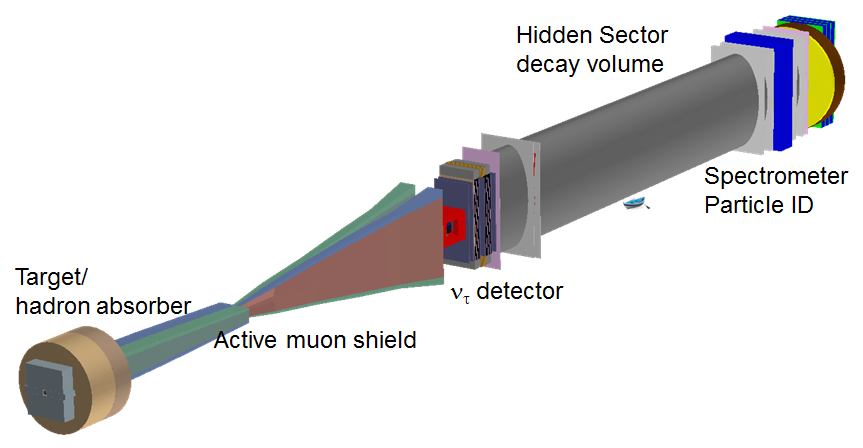
\includegraphics[width=0.9\textwidth]{introduction/SHiP-facility-overview}
	\caption{Overview of the SHiP facility \cite{ship_TP} }
	\label{fig:detector-overwiew}
	\end{figure}
	
	The detector for the direct detection of the hidden particles is designed to fully reconstruct their exclusive decays. Table \ref{table:req_decaymodes} summarizes the main decay modes of the hidden particles in the various models considered.
	
	\begin{table}[htb]
\begin{center}
\caption{Summary of the main decay modes of hidden particles in various models ($\ell = e, \mu$).}
\label{table:req_decaymodes}
\vspace{2mm}
\begin{tabular}{ll}
\hline
Models                         	& Final states              \\
\hline
Neutrino portal, SUSY neutralino                 & $\ell^{\pm}\pi^{\mp}, \ell^{\pm} K^{\mp}, \ell^{\pm}\rho^{\mp},\,\,\,\,\, \rho^{\pm}\rightarrow \pi^{\pm}\pi^0$ \\
Vector, scalar, axion portals, SUSY sgoldstino   & $\ell^+\ell^-$ \\
Vector, scalar, axion portals, SUSY sgoldstino   & $\pi^+\pi^-, K^+K^-$ \\
Neutrino portal ,SUSY neutralino, axino          & $\ell^+\ell^-\nu$ \\
Axion portal, SUSY sgoldstino                    & $\gamma\gamma$ \\
% Axino ?                                          & $\gamma$... \\ 
SUSY sgoldstino                                  & $\pi^0\pi^0$ \\
\hline
\end{tabular}
\end{center}
\end{table}

	The principal background to the hidden particle decay signal originates from the inelastic scattering of neutrinos and muons in the vicinity of the detector producing long-lived particles.
	
	The beam line is designed to minimize the background sources. The proton
interaction in the target gives rise to a copious direct production of short-lived resonances, pions and kaons. While a hadron stopper of a few metres of iron is sufficient to absorb the hadrons and the electromagnetic radiation emerging from the target, the decays of pions, kaons and short-lived resonances result in a large flux of muons and neutrinos. In order to reduce the flux of neutrinos, in particular the flux of muon neutrinos and the associated muons, the pions and kaons should be stopped as efficiently as possible before they decay. The target must therefore be made of a material with the shortest possible interaction length and be sufficiently long to contain the hadronic showers with minimum leakage. Since the production angle of the  hidden particles is relatively large, there is no requirement to minimize the beam spot.

	The short-lived resonances and the residual flux of decaying pions and kaons still give rise to a large flux of muons. This flux must be efficiently cleared from the detector fiducial volume by either a passive shield or through an active shield based on magnetic deflection. The residual flux should also be low enough so not to compromise the occupancy limit in the tau neutrino detector. As illustrated in Figure \ref{fig:detector-overwiew}, in the baseline design a 5 m horizontally wide region respecting these requirements has been achieved with a 48 m long active muon shield based on magnetic deflection of the muons in the horizontal plane.
	 
	The muon shield is followed by the 10 m long tau neutrino detector, which puts the start of the HS decay volume at about 64 m \cite{ship_TP}. The main purpose of the tau neutrino detector is to perform the first direct observation of the $\overline{\nu}_\tau$, and to study the properties and the cross section of $\nu^\tau$ and $\overline{\nu}_\tau$.
 The current optimization of muon shield and cost, results in a decay volume with an elliptical shape of 5 m width and 10 m height. The length of the decay volume is obtained by maximizing the acceptance to the hidden particle decay products given the transversal size.

	The full reconstruction of the hidden particle decays requires a magnetic spectrometer and a system for particle identification at the end of the decay volume.
	
	The particle identification system requires an electromagnetic calorimeter for $e / \gamma$ identification with sufficient granularity and energy resolution in order to reconstruct $\pi^0$'s, and a hadron calorimeter in combination with a muon detector for $ \pi / \mu$ separation.
	
	\begin{figure}[!h]
	\centering
	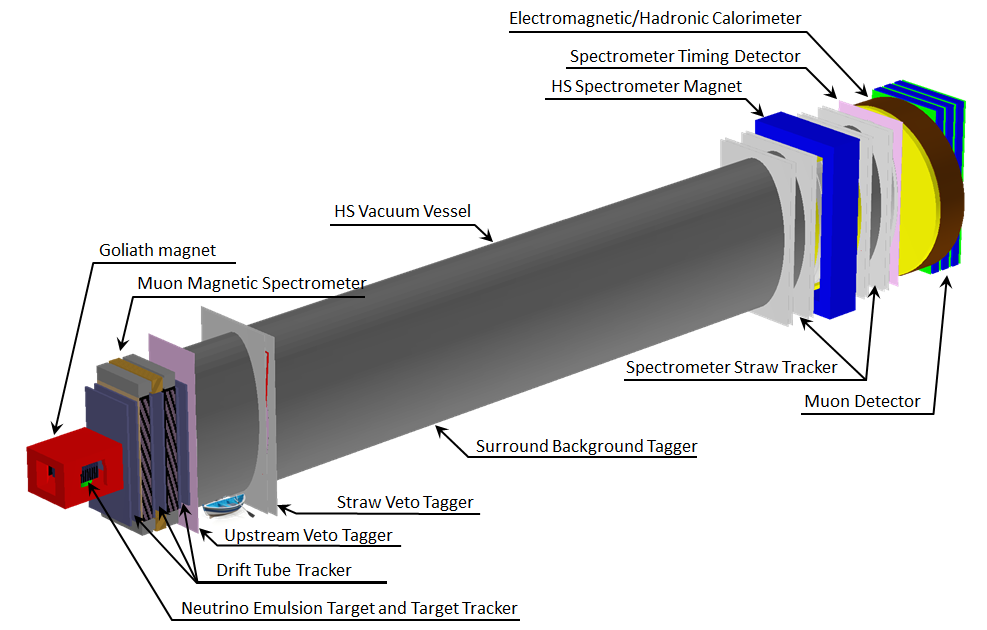
\includegraphics[width=\textwidth]{SHiP-detector-overview}
	\caption{SHiP detector layout}
	\end{figure}
	
	\subsection{Spectrometer tracker}
	
	Spectrometer tracker is a part of particle identification system.  The purpose of the HS spectrometer is to reconstruct with high efficiency the tracks of charged particles from the decay of hidden particles. The spectrometer must provide an accurate determination of the track momentum and of the flight direction within the fiducial decay volume.
	
	\begin{figure}[h!]
		\centering
		\subfloat[Position of the tracking stations and dipole magnet, overlaid with magnetic field component $B_x$ as a function of z.]{
			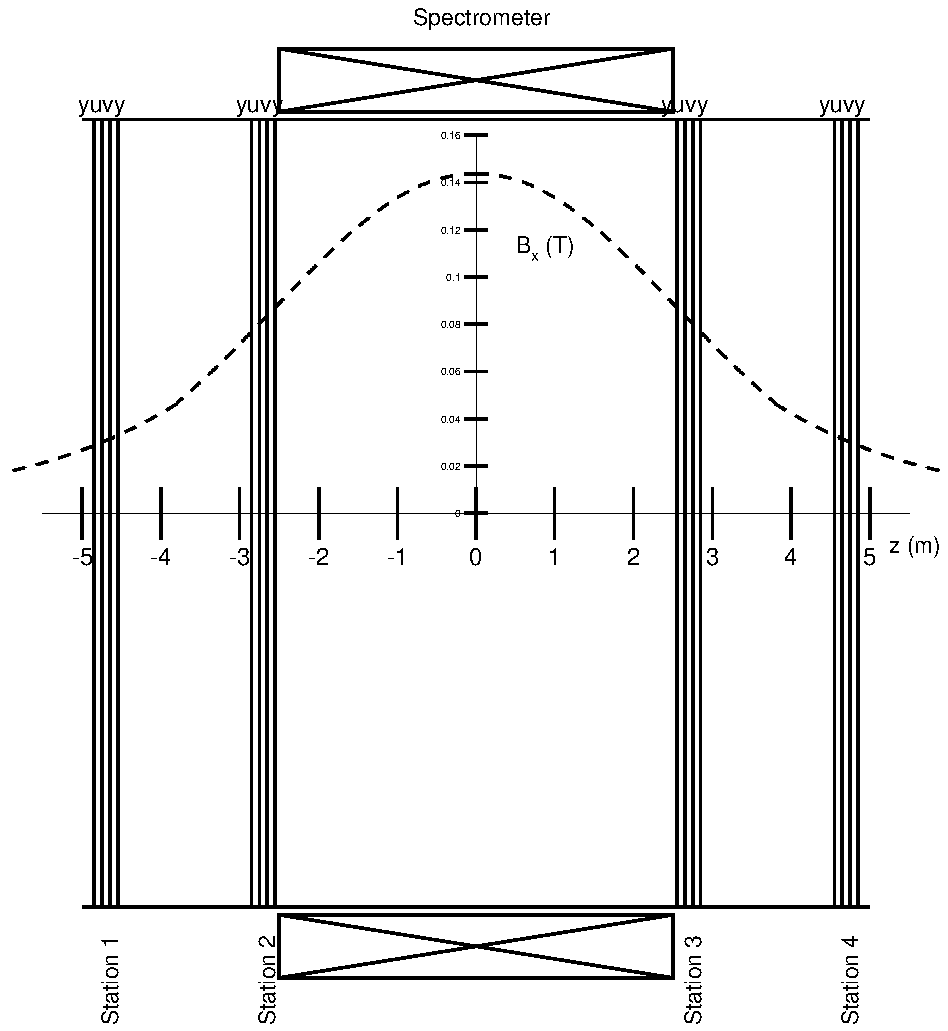
\includegraphics[width=0.50\textwidth]{introduction/spectrometer-layout} 
			\label{fig:spectrometer_layout} }%
		\qquad
		\subfloat[Four views in one station (not all straws shown, for the sake of clarity). The nominal acceptance, defined by the vacuum vessel, is shown as a red ellipse.]{
			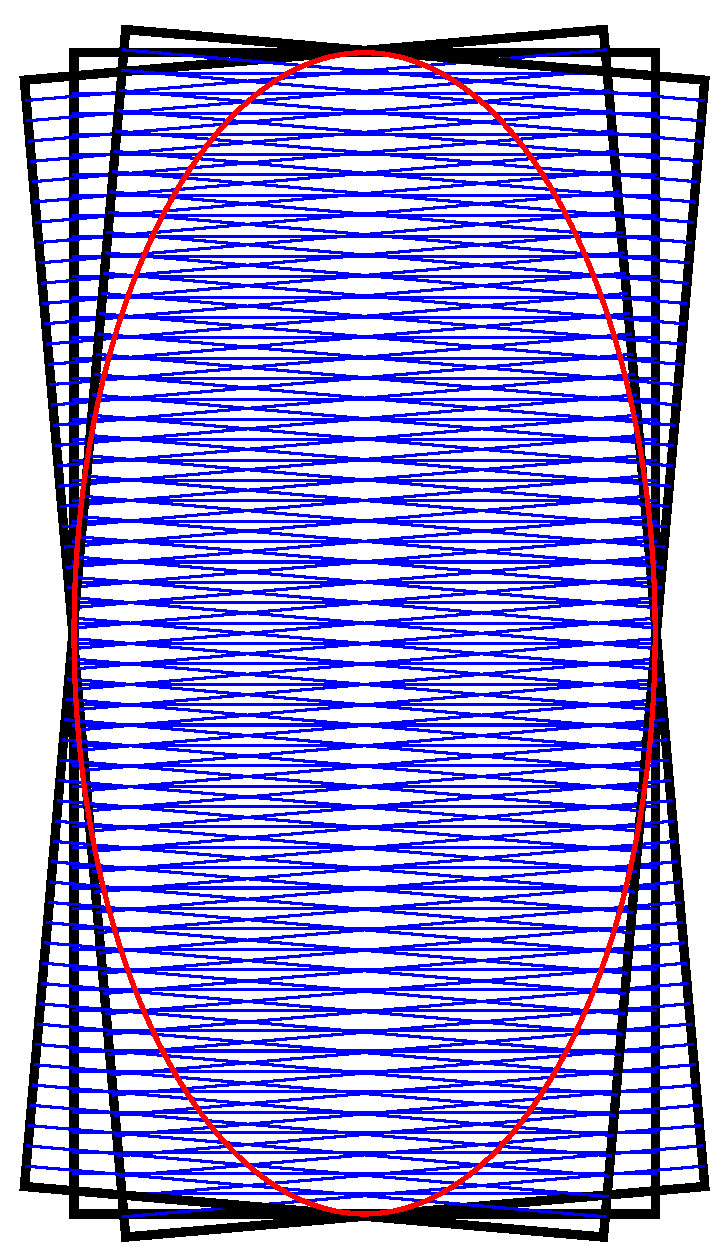
\includegraphics[width=0.4\textwidth]{introduction/straw-views.pdf} 
			\label{fig:cluster_distrib} }%
		\caption{Spectrometer layout}
	\end{figure}

	
	The spectrometer consists of a large aperture dipole magnet and two tracking telescopes on each side of the magnet. A layout with four tracking stations
symmetrically arranged around the dipole magnet, as depicted in Figure \ref{fig:spectrometer_layout}, is taken as a baseline. The size and layout of the tracker stations is connected to the size of the magnet. A dipole spectrometer magnet with a horizontal gap of 5 m, a height of 10 m and a length of 5 m provides good acceptance coverage and is considered feasible at a reasonable cost.

	Following the direction of the magnetic field, the measuring elements are oriented horizontally to measure precisely the vertical (Y) coordinate. Two stereo views (U and V) are rotated by an angle $ \pm \theta _{stereo}$ for measuring the transverse coordinate X with an accuracy degraded by $ \sim 1/ \sin \theta _{stereo}$. The precision in X (i.e. the value of the stereo angle) is driven by the need of a good enough measurement of the decay vertex, opening angle of the daughter particles (which enters the invariant mass) and impact parameter at the production target. Each station contains 4 views (Y-U-V-Y). The two stations on the same side of the magnet are separated by $\bigtriangleup = 2 m$ and a gap of $5 m$ is left between the second and third stations (i.e. each is $2.5 m$ away from the centre of the magnet).
	
	The tracking stations of the magnetic spectrometer must provide good spatial resolution and minimise the contribution from multiple scattering. In addition, the tracker must operate in vacuum. A straw tracker made of thin polyethylene terephthalate (PET) tubes is ideal to meet these goals. Gas tightness of these tubes has been demonstrated in long term tests and the mass production procedure is also well established (see NA62 experiment \cite{NA62_TDR}). The main differences between the SHiP tracker and the NA62 tracker are the need for $5 m$ long straws (vs 2.1 m in NA62). The main changes with respect to the Expression of Interest \cite{EoI} follow from the changes applied to the spectrometer magnet. The straw orientation has been turned from vertical to horizontal and one transverse dimension has been increased from 5 to 10 m.
	
%	\end{spacing}	

	 \section{Subject of study}
	
	With new requirements for new straw tracker we have important challenge for long straws. It  is related with the fact that straw and wire will be subjected to gravitational and electrical forces and it causes the sagging. Because the straws are oriented horizontally (or almost, in case of stereo views), sagging is expected to cause in most drift tubes a downward deflection, which might be exploited
when applying a correction.

	Undoubtedly the presence of sagging can complicate the data processing stage and somewhat worse accuracy of track reconstruction. Primary question we have to investigate "is acceptable sag-admitting design?" and "What a downgrade of precision for sag-admitting design?".
	
	Results of measurements on prototypes are discussed in Section \ref{sec:Mesurements}.
	

	\section{Signal}
	Computer program Garfield \cite{garfield} is designed for detailed simulation of two- and three-dimensional gas detectors. So we will perform STRAW tube studies using this program.
	
	Charged particle  create electron-ion pairs wile traverse the drift tube. Electrons under affecting the electric field drift to the wire anode (see Fig.\ref{fig:track_reconstruction}). During the travel they increase their energy and invoke an avalanche. Therefore they produce a measurable signal.

	Initial electrons drift to the wire due to the electrical field between the wire and the tube wall. Electrons ionize gas molecules due to the high electric field around the wire, especially near the wire when the strength of the electric field becomes very large.  Subsequently readout electronics process the signal induced on the wire.
	  
	The event is registered if signal reach some a threshold voltage (Fig. \ref{fig:signal_example}). So the value of threshold is a key factor on the way of searching optimal setting for signal processing procedure.
	
	\begin{table}[h]
	\centering
	\caption[Table caption text]{STRAW tube parameters }
	\begin{tabular}{|l|l|p{8cm}|}
		\hline
		parameter name & value \\
		\hline
		wire & $30~\mu m$ gold-plated Tungsten\\
		\hline
		straw length & $5~m$ \\
		\hline
		voltage & $1750~V$ \\
		\hline
		inner tube radius & $9.8~mm$ \\
		\hline
		wire medium density & $19.3 ~g/cm^3$ \\
		\hline
		wire tension& $\sim 90~g$ \\
		\hline
		working tube gas mixture & $Ar~70\% ~CO_230\%$ \\
		\hline
	\end{tabular}
	
	\label{table:straw_par}
	\end{table}		
	
	We have to set threshold as low as possible but enough above from noise level to achieve best rate of true/false detected tracks and highest track registration precision and efficiency.
	
	A variation of the signal height introduces a variation in the time when the signal passes the threshold and is considered to be the main contribution to the STRAW tracker resolution. 
	
	\begin{figure}[!h]
	\centering
	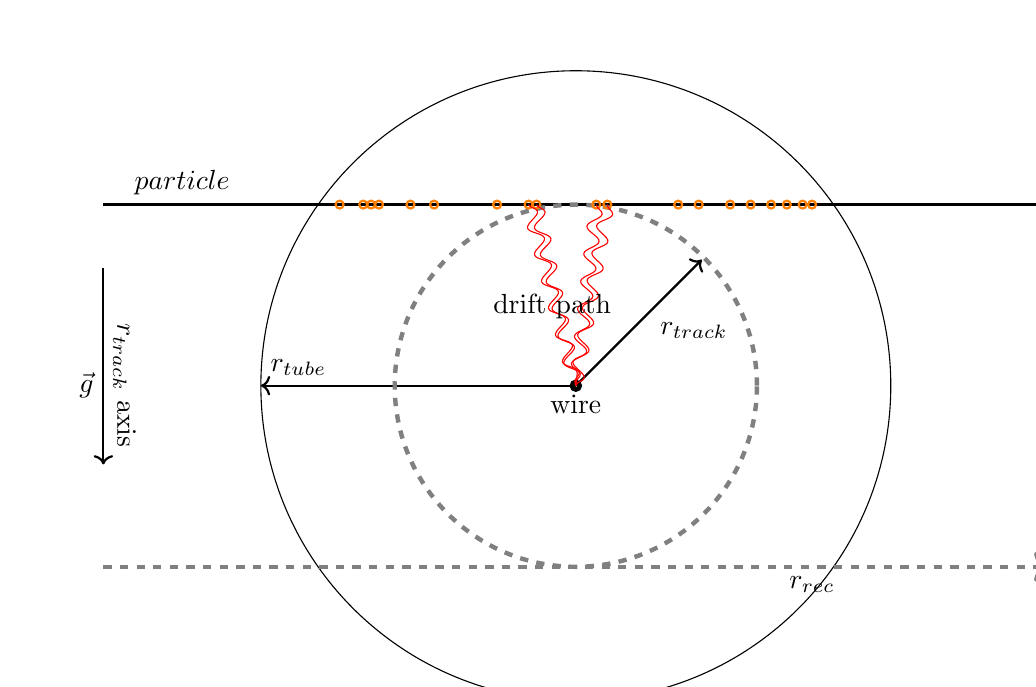
\begin{tikzpicture}
	
	\tikzset{snake it/.style={decorate, decoration=snake}}
	
	\draw (0,0) circle (4);
	
	\draw[ultra thick] (0,0) circle (0.05);
	\node[below] at (0,0) {wire};
	
	\draw[thick,->] (0,0) -- (1.6,1.6);	
	\node at (1.5,0.7) {$r_{track}$};

	\draw[thick,->] (0,0) -- (-4,0);	
	\node[above right] at (-4,0) {$r_{tube}$};
		
	\draw[thick,->] (-6,2.3) -- (6,2.3);
	\node[above] at (-5,2.3) {$particle$};
	
	\draw[ultra thick, gray, dashed, ->] (-6,-2.3) -- (6,-2.3);
	
	\draw[ultra thick,gray,dashed] (0,0) circle (2.3);
	\node[below] at (3,-2.3) { $r_{rec}$};
	
	% gravitation force vector
	\draw[thick, ->] (-6,1.5) -- ( -6, -1);
	\node[left] at (-6,0) {$\vec{g}$};
	
	% r_track axis
	\node[above,rotate=-90] at (-6,0) {$r_{track}$ axis};
	
	% initial ekectron/ion clusters
	\draw[thick,orange] (-3.0,2.3) circle(0.05);
	\draw[thick,orange] (-2.7,2.3) circle(0.05);
	\draw[thick,orange] (-2.6,2.3) circle(0.05);
	\draw[thick,orange] (-2.5,2.3) circle(0.05);
	\draw[thick,orange] (-2.1,2.3) circle(0.05);
	\draw[thick,orange] (-1.8,2.3) circle(0.05);
	\draw[thick,orange] (-1.0,2.3) circle(0.05);
	\draw[thick,orange] (-0.6,2.3) circle(0.05);
	\draw[thick,orange] (-0.5,2.3) circle(0.05);
	\draw[thick,orange] (0.26,2.3) circle(0.05);
	\draw[thick,orange] (0.4 ,2.3) circle(0.05);
	\draw[thick,orange] (1.3 ,2.3) circle(0.05);
	\draw[thick,orange] (1.56,2.3) circle(0.05);
	\draw[thick,orange] (1.96,2.3) circle(0.05);
	\draw[thick,orange] (2.22,2.3) circle(0.05);
	\draw[thick,orange] (2.48,2.3) circle(0.05);
	\draw[thick,orange] (2.68,2.3) circle(0.05);
	\draw[thick,orange] (2.88,2.3) circle(0.05);
	\draw[thick,orange] (3.00,2.3) circle(0.05);
	
	\draw[red,snake it](-0.6,2.3) -- (0,0);
	\draw[red,snake it](-0.5,2.3) -- (0,0);
	\draw[red,snake it](0.26,2.3) -- (0,0);
	\draw[red,snake it](0.4,2.3) -- (0,0);
	\node[] at (-0.3,1) {drift path};
	
	\end{tikzpicture} 
	\caption{Schematic view of a particle passing the straw and producing
ionization clusters (orange points). Electrons of ionization cluster drift to the wire and induce the signal. The closest distance from the track to the wire, $r_{track}$, and radius of the straw, $r_{tube} = 2.45 mm$, are also indicated. }
	\label{fig:track_reconstruction}
	\end{figure}


	In the track reconstruction software(GARFIELD \cite{garfield}) an effective TR-relation is used. It only describes the relation between the drift time and the distance from the track to the wire, which differs from the distance to the ionization cluster. The shape of the TR-relation is defined by the drift velocity of the ionization cluster inside the straw. The electric field increases towards the wire, leading to a non linear TR-relation. 

	The drift time versus the unbiased distance distribution and the result of the fit are shown in Fig. \ref{fig:t_r_distr_00}. Noise hits under the main distribution, i.e. at earlier times, are due to primary or secondary particles ($\delta$-rays) passing the straw at a closer distance to the wire, consequently producing an earlier signal. Initial clusters along the track are marked by orange points in the figure.
	
	Muon $\mu$ was chosen as test particle for simulation with energy $1GeV$. You can see some of typical tracks from the $\mu$ through the tube Fig.\ref{fig:electron_ion_track},\ref{fig:electron_ion_track_sag}. 
			
	
	\subsection{ Leakage noise}
	Every time we deal with different kind of noise. Basically it is noise from  leakage current through readout electronics.

	As will be discussed further we analyse not the current invoked by particle but the output voltage from amplifier. In GARFIELD we able convolute input current $I(t)$ with electronic response function (\ref{eq:responce_function}) \footnote{in this equation $t$ in nanoseconds} 
	
	\begin{equation}
	f_{resp} =  A\cdot(e^{-t/0.005} - e^{-t/0.030})
	\label{eq:responce_function}
	\end{equation}
	
	Noise is very important for every calculations and it makes bit impact on straw precision and straw efficiency. So we can't rely on results until we receive signal and noise  from real STRAW tube prototypes. 
		
	Convolution of input current makes it smooth. Usually in typical conditions\footnote{as in table \ref{table:straw_par}} noise have gauss distribution with RMS equal to a amplitude of signal from 2000 electron in the tube - electric noise charge (ENC)\footnote{With testing of real 5 m long straws and ultimate examples of electronics we will measure real noise. But for now it is only close to reality suggestion concerning to this issue.} On Fig.\ref{fig:signal_example} you can see deposition from noise marked by blue line.

	On the Fig.\ref{fig:signal_example} the timestamp $Time=0$ corresponds to the time when muon hits a tube. The convolution function smooths and spreads input current. It mean that the output voltage in GARFIELD does not contain part of signal before hit event timestamp.

	\begin{figure}[h!]
	\centering
	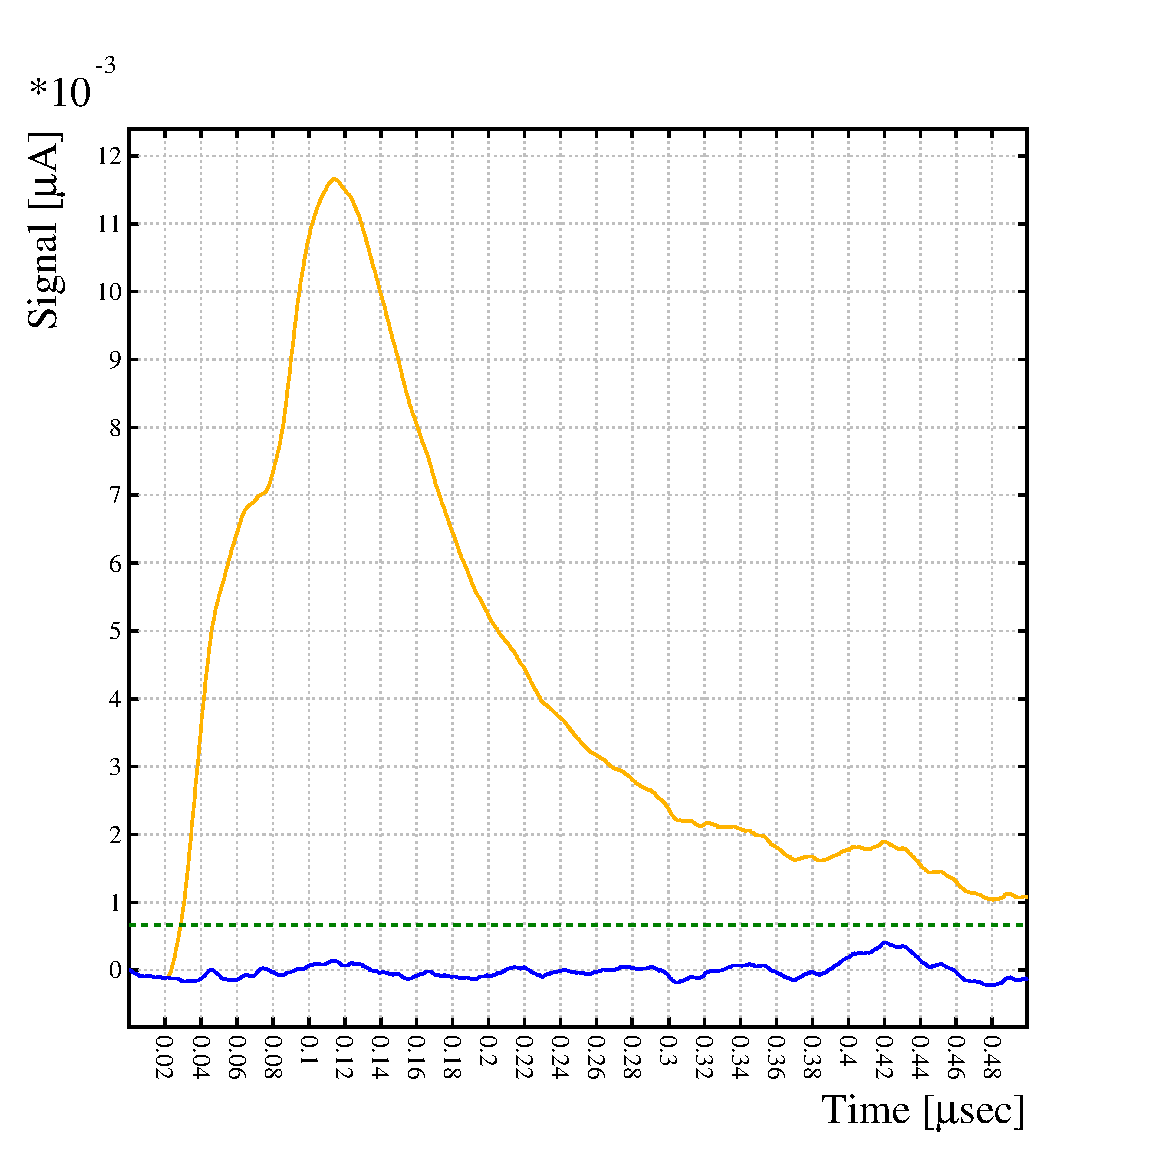
\includegraphics[width=0.7\textwidth]{signal_noise_threshold.eps}
	\caption{ Example of output signal $V(t)$ after convolution (front-end electronics) from central track (yellow line). The noise component of the same signal depicted by separate blue line. Grin dashed line is a threshold for trigering drift time and equals to $5\sigma$ of noise distribution.}
	\label{fig:signal_example}
	\end{figure}
	
	\subsection{ STRAW efficiency}
	
	The interaction of charge particle with gas molecules has probabilistic nature. For short distance tracks (somewhere near the tube wall) the probability of tracks that generation of zero electron/ion pairs becomes significantly high.
	
	The number of produced ionization clusters directly affects the hit efficiency profile. Smaller ionization length increases the hitting efficiency because of production more ionization clusters per length unit \cite{kozlinskiy}. In GARFIELD we can easily calculate amount of clusters per track. In Fig.\ref{fig:cluster_distrib} you can see a distribution of number of clusters per central track for our STRAW tube. It means that straw efficiency will be lower near the tube wall (see Fig.\ref{fig:efficiency}).
		

	\begin{figure}[h!]
	\centering
	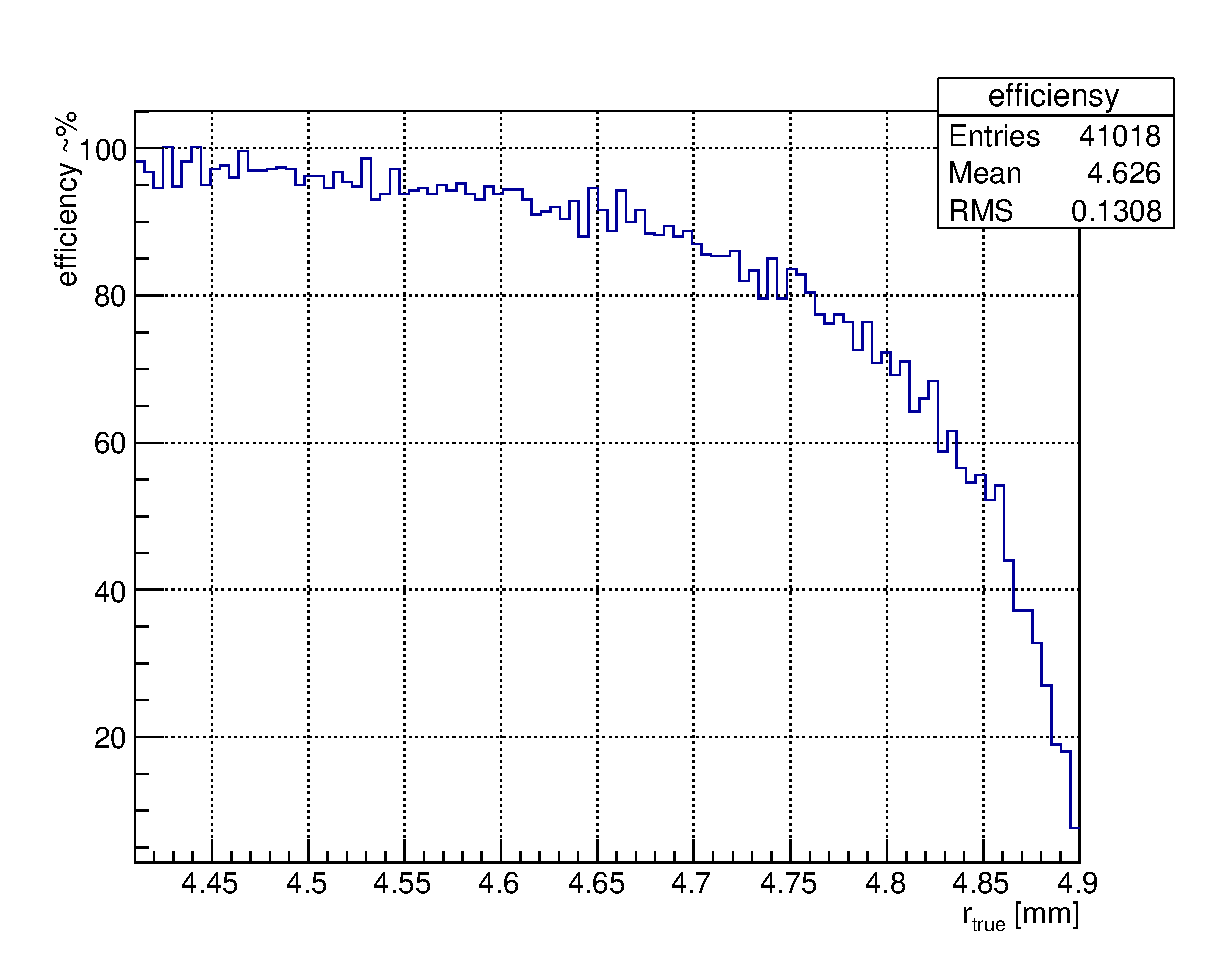
\includegraphics[width=0.8\textwidth]{periffEff}
	
	\caption{Straw tube efficiency. Result of homogeneous penetrating periphery of tube by 50k events (scaled down by factor of 5. $\dfrac{50k~events}{100 bin}  = 500 \dfrac{eventst}{bin}$).}
%	Ефективність реєстрації треків в області периферії трубки від рівномірного опромінення 50 тис. треків
	\label{fig:efficiency}
	\end{figure}	
	
	\begin{figure}[h!]
		\centering
		\subfloat[electrons per cluster]{
			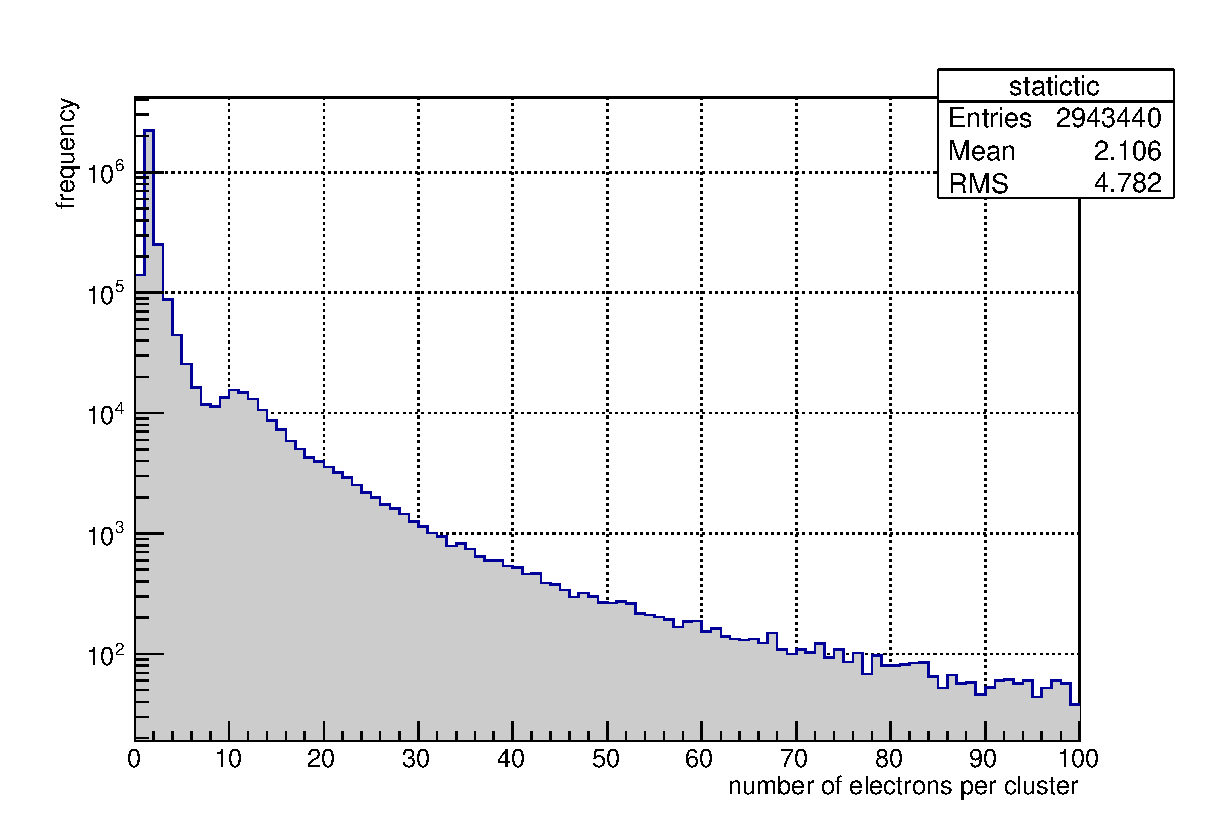
\includegraphics[width=0.45\textwidth]{el_per_cluster} 
			\label{fig:el_per_cluster} }%
		\qquad
		\subfloat[number of clusters per central track]{
			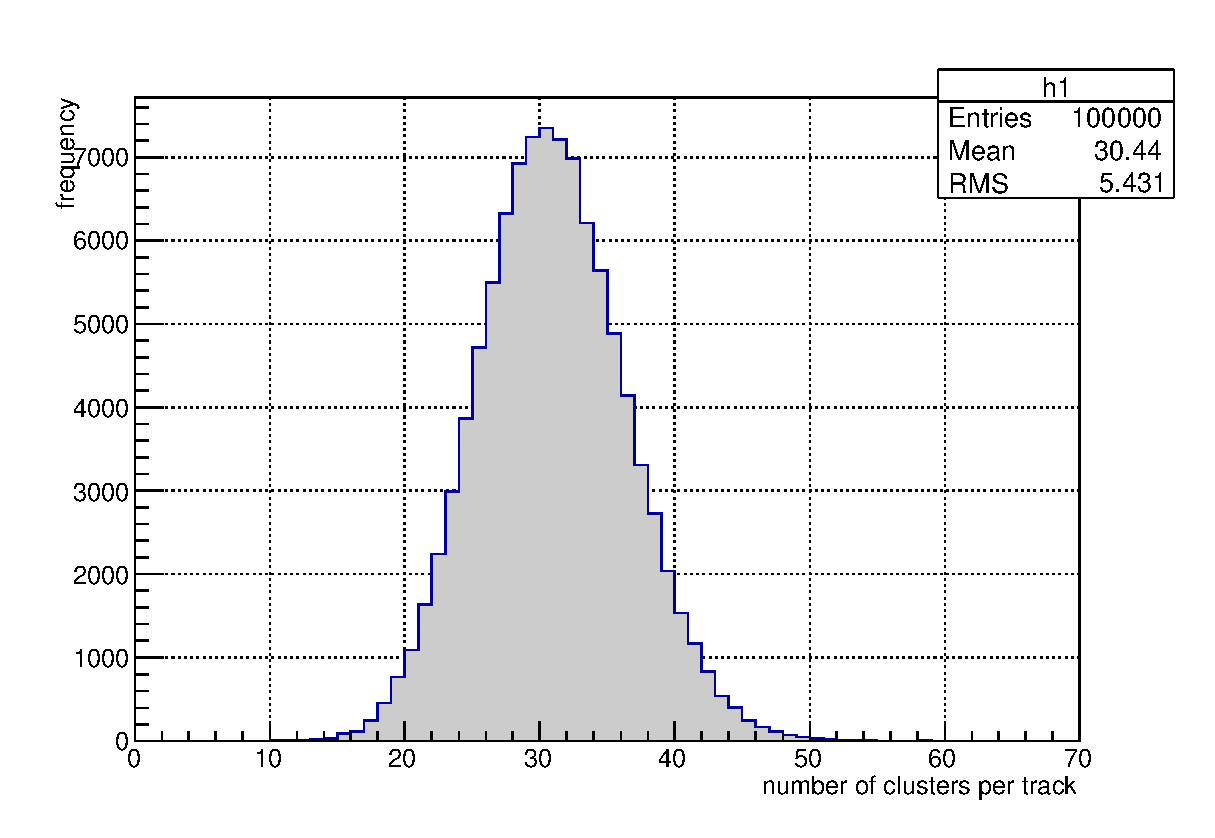
\includegraphics[width=0.45\textwidth]{cluster_distrib} 
			\label{fig:cluster_distrib} }%
			\caption{Statistics info from GARFIELD about track from $1GeV~\mu$. Tube described in table~\ref{table:straw_par}}
	\end{figure}
	
	From the Fig.\ref{fig:efficiency} we can conclude that the efficiency of tube is $100\%$ almost in whole region covered by tube except pre wall region which is quite small. Increasing the gas mixture density or increasing the tube radius for the same gas density can increase tube efficiency.
	
		\section{Gain}
	
	Lets look on avalanche process in the tube. If multiplication occurs, the increasing of the number of electrons per path $ds$ is given by
	
	\begin{equation}
		dN = N \alpha ds
		\label{eq:diffGain}
	\end{equation}
	
	The coefficient $\alpha$ is determined by the excitation and ionization cross sections of the electrons that have acquired sufficient energy in the field. It also depends on the various transfer mechanisms and electric field E and increases with the field because the ionization cross-section goes up from threshold as the collision energy $\varepsilon$ increases. As we can suppose the coefficient $\alpha$ is of big amount of parameters.
	
	The amplification factor $G$ on a wire(that is more interesting for us) is given by integrating (\ref{eq:diffGain}) between the point $s_{min}$ where the field is just sufficient to start the avalanche and the wire radius $a$:
	
	\begin{equation}
	G = N/N_0 = exp \int\limits_{s_{min}}^{a} \alpha(s) ds
	\label{eq:gain}
	\end{equation}
	
	GARFIELD can provide us by amplification factor $G$ for any point of the tube(because  $G$ is coordinate dependent magnitude). The amplification factor is equal almost in whole tube space except neighbourhood near the wire because electric field  becomes significantly high only near the wire (see figs \ref{fig:elFieldCentered}, \ref{fig:elField1mmShifted}). When the wire is shifted from the center of the tube the electric field in area close to the wire is the same as in centered state. So the amplification factor $G$ is quite similar in both cases.
	
	\begin{figure}[!h] 
		\centering
		\subfloat[electric field for centered wire]{
			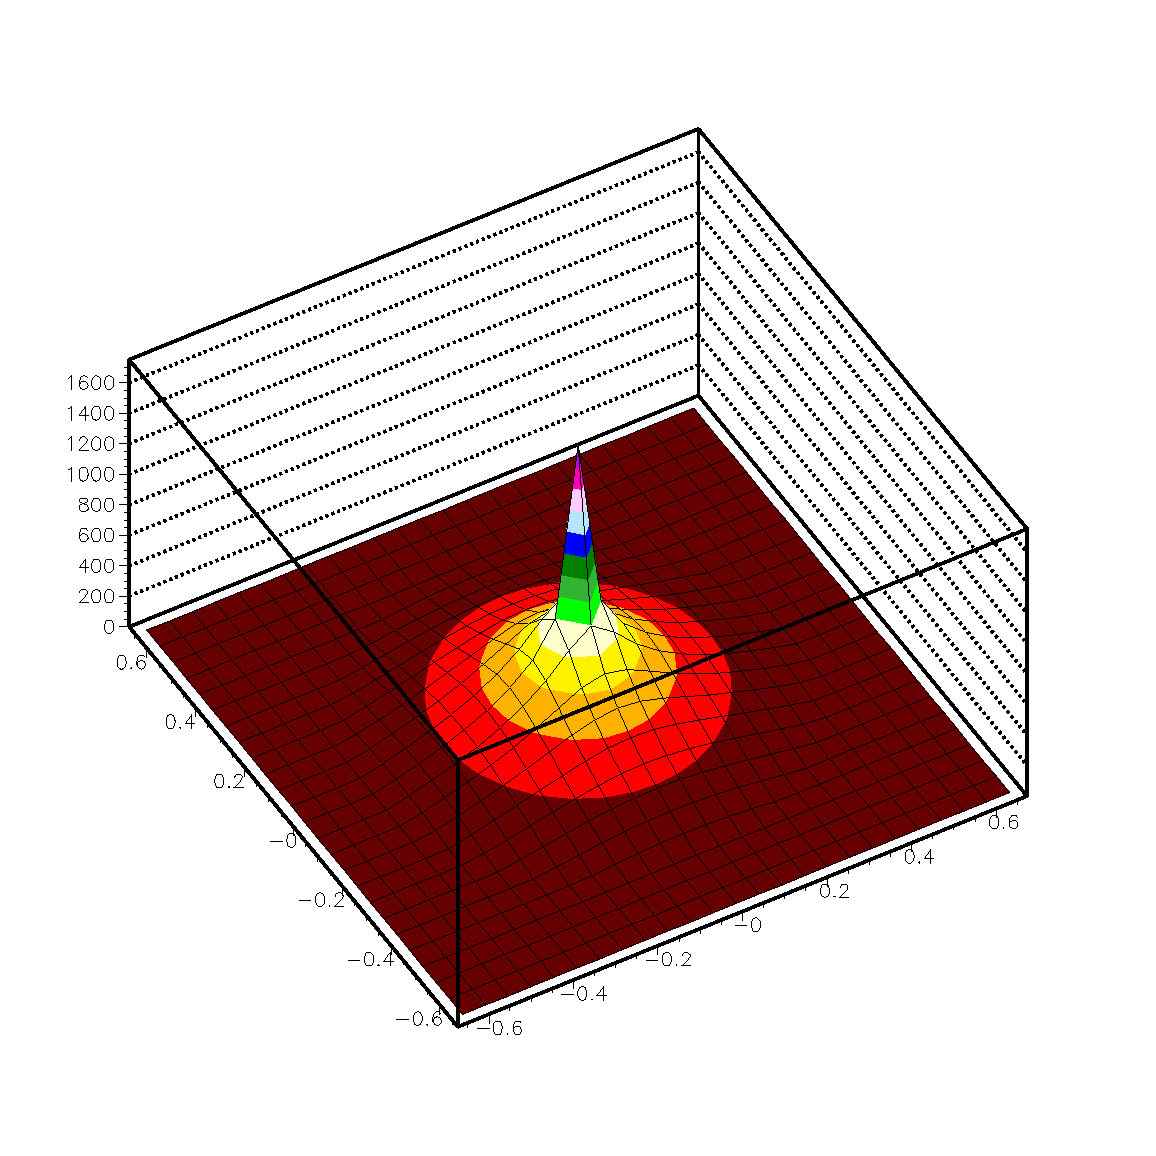
\includegraphics[width=0.45\textwidth]{fieldCentered} 
			\label{fig:elFieldCentered} }%
		\qquad
		\subfloat[electric field for $1 mm$ shifted wire]{
			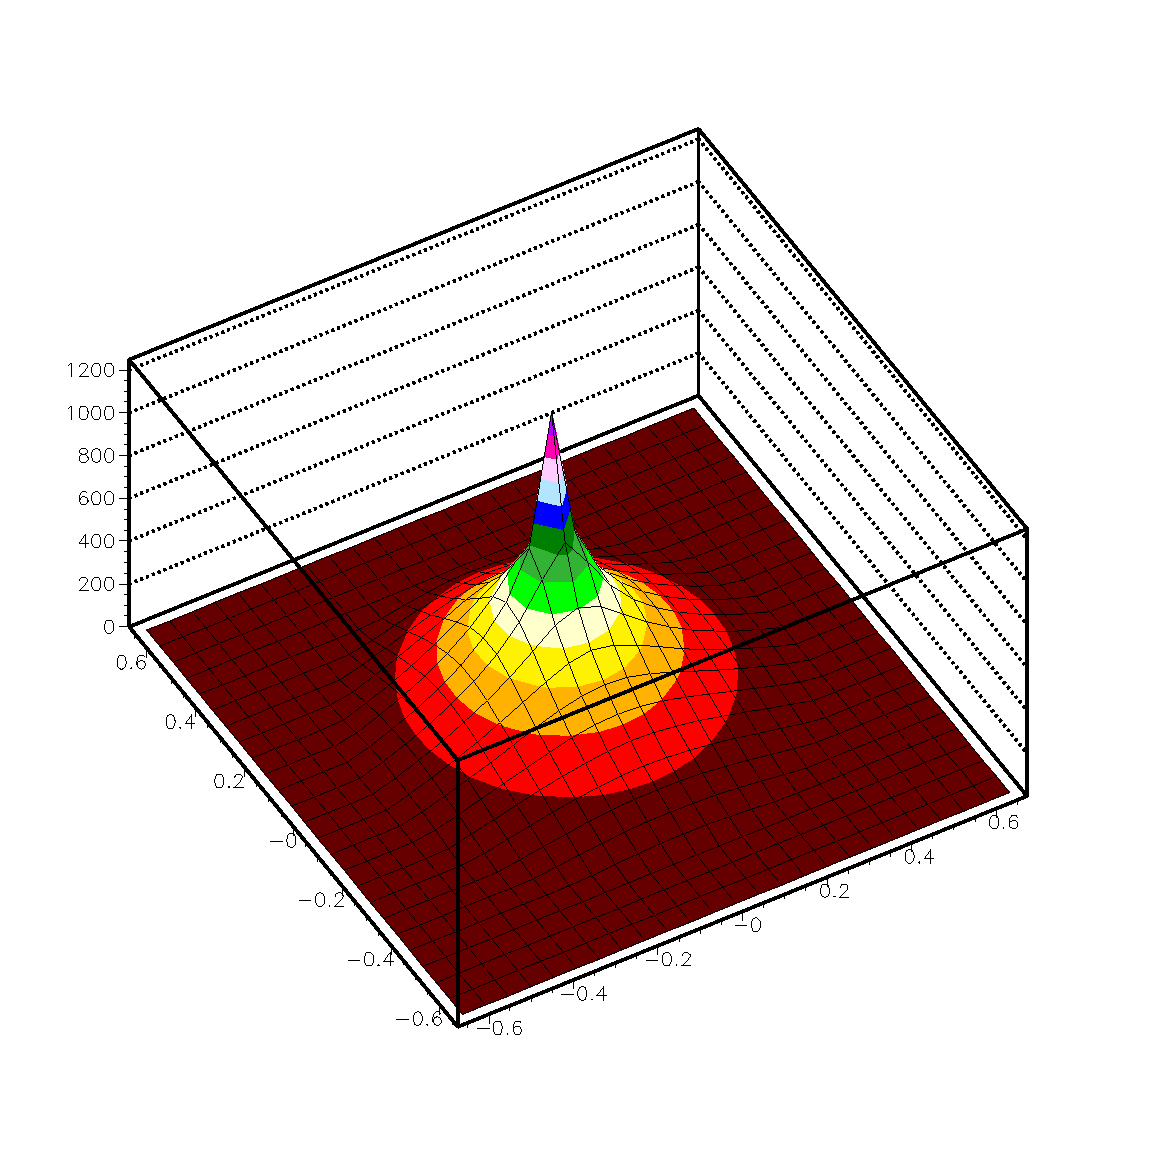
\includegraphics[width=0.45\textwidth]{field_10Sag}
			\label{fig:elField1mmShifted} }%
		\caption{Electric field intensity map for different wire position in the cube calculated in GARFIELD software. Conditions for those plots are described in table \ref{table:straw_par} }
	\end{figure}
	
	Implementation of gain value calculation is not so reliable in GARFIELD(especially fortran version). Gain should be recalculated using Garfield++ (which is newer and takes into consideration more effects). 
	
	\begin{figure}[h!]
	\centering
	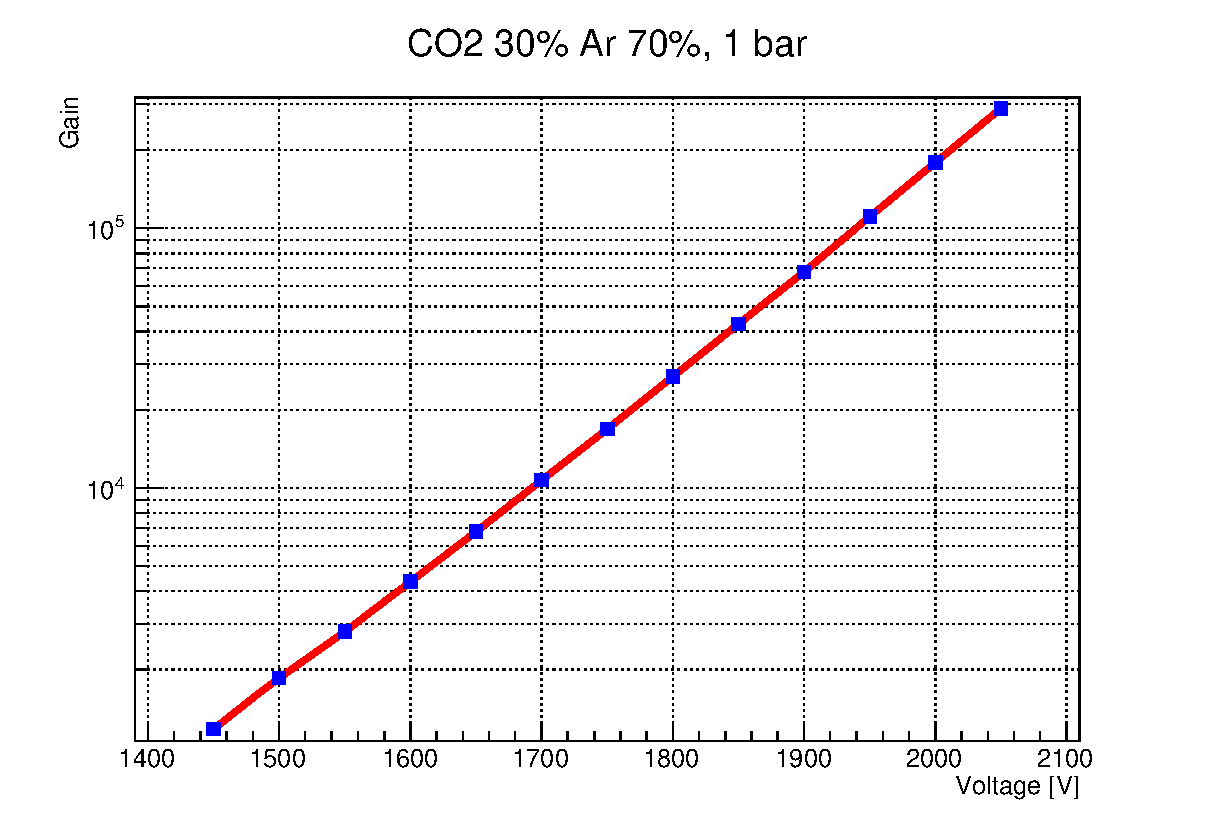
\includegraphics[width=0.7\textwidth]{gain_1450_2050V}	
	\caption{Dependence of the gain of the voltage applied to the wire. The rest of STRAW tube settings corresponds to table \ref{table:straw_par}. }
	\label{fig:gainVoltage}	
	\end{figure}

	On the Fig.\ref{fig:gainVoltage} you can see that the gain $G(V)$ have precisely exponential dependence. This is frankly does not inspire confidence. The difference can be up to 100\% (as Rob Veenhof - creator of GARFIELD \cite{garfield} said).
			 

	\section{Wire sagging}

	Easy to predict that the displacement of the wire invokes distortion an electric field (see figs~\ref{fig:elFieldCentered},\ref{fig:elField1mmShifted}) and drift path for electrons/ions inside the tube (see fig.\ref{fig:electron_ion_track} and Fig.\ref{fig:electron_ion_track_sag}). The RT-relation for track reconstruction directly depends on the wire position in the tube. So RT-relation loses it's previous symmetry (see next sections).
	
	\begin{figure}[h!]
		\centering
		\subfloat[wire in the center of the tube]{
			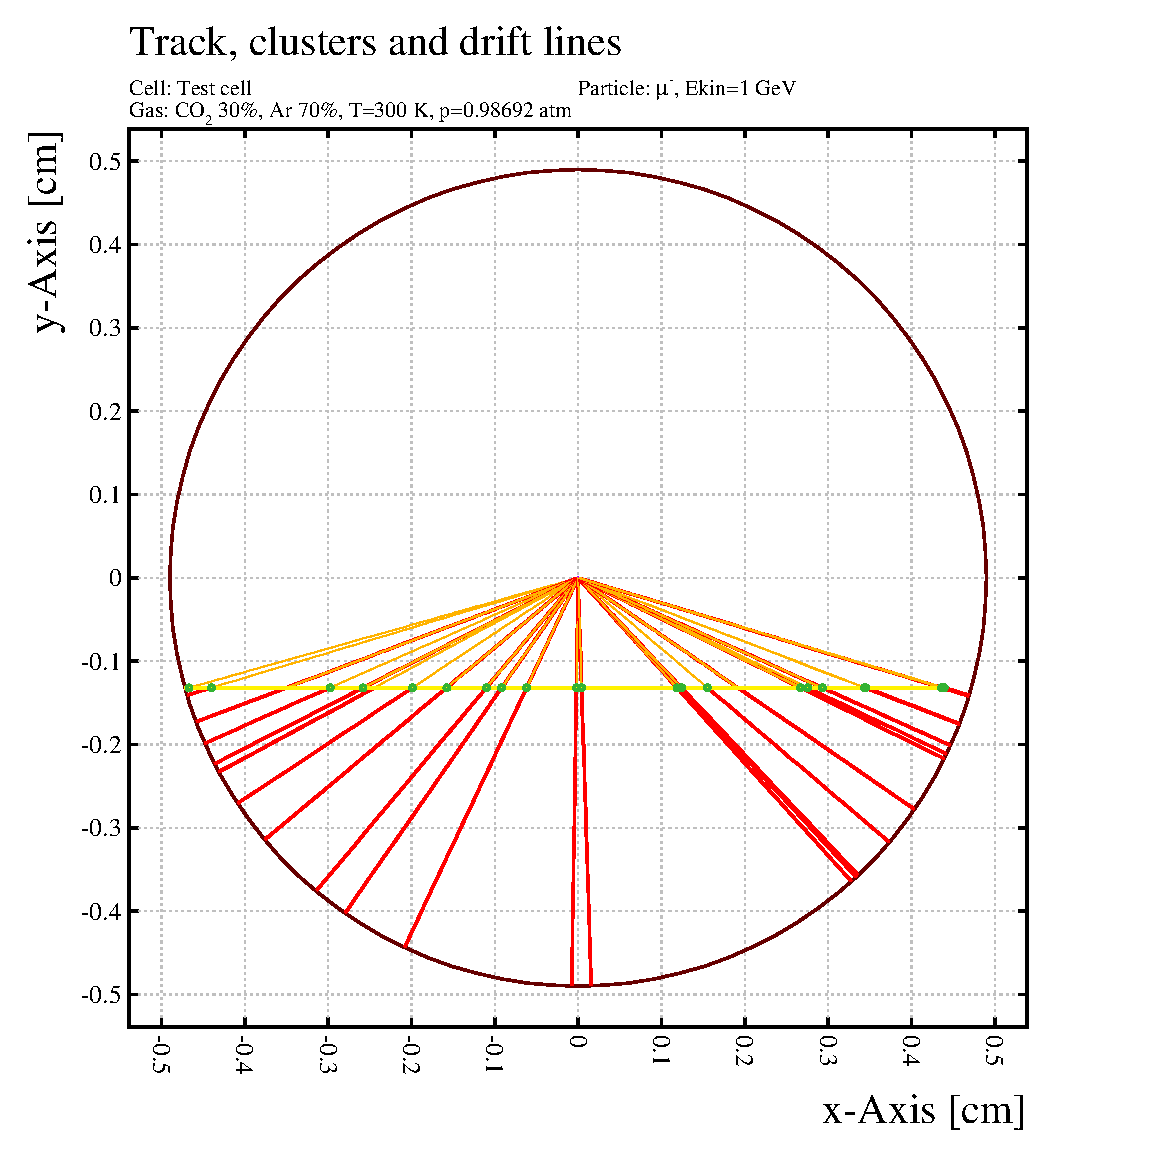
\includegraphics[width=0.45\textwidth]{sag/tracksAndClusters00Sag.eps} 
			\label{fig:electron_ion_track} }%
		\qquad
		\subfloat[sagging $1.5 mm$]{
			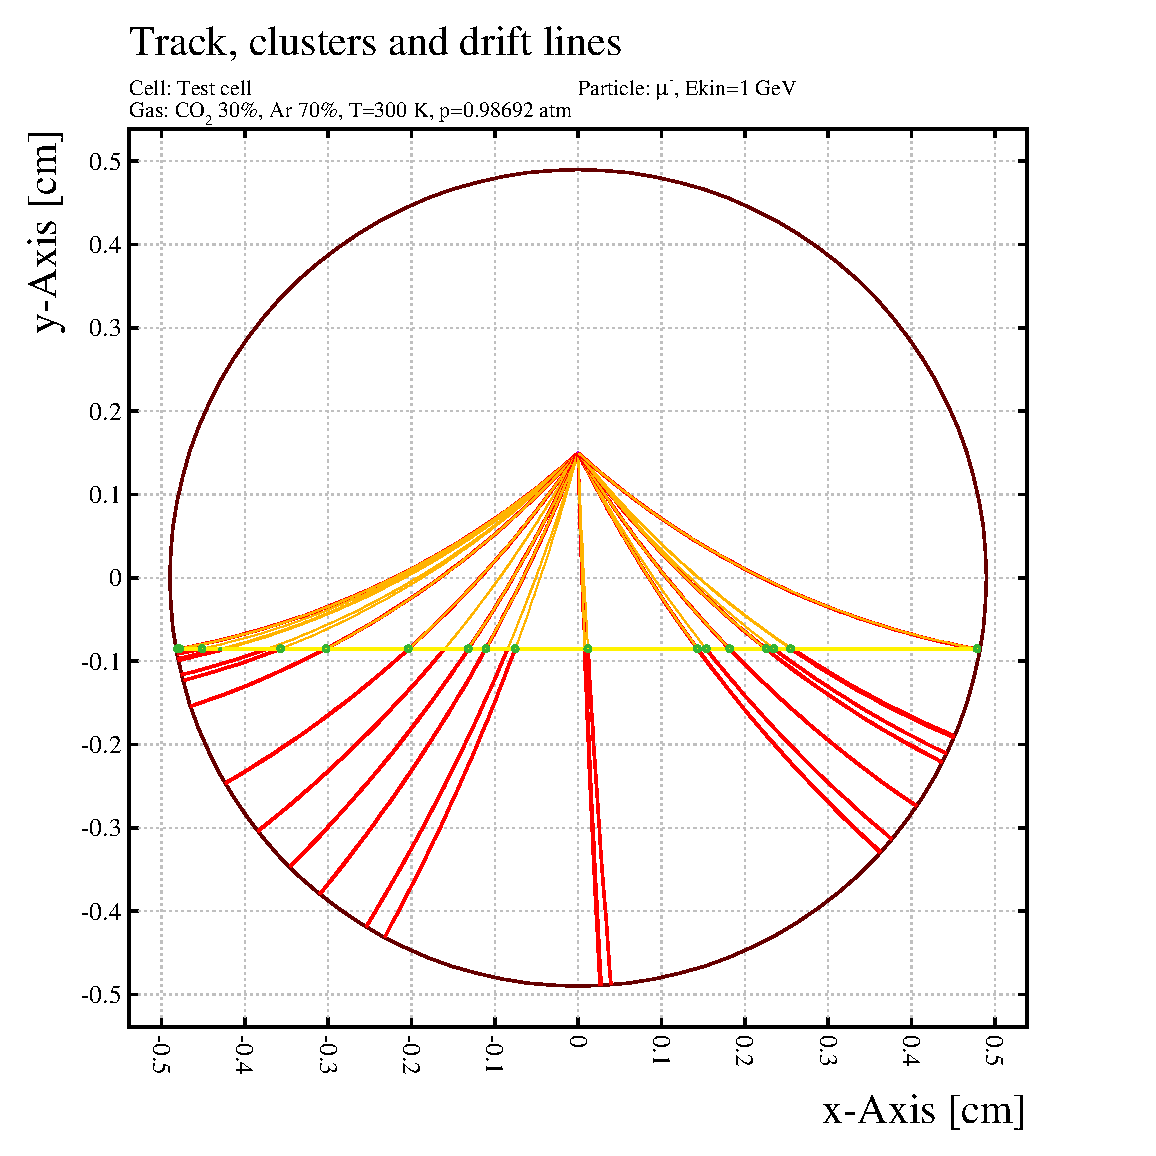
\includegraphics[width=0.45\textwidth]{sag/tracksAndClusters15Sag.eps} 
			\label{fig:electron_ion_track_sag} }%
		\caption{ An example of tracks from the on the tube for different position of the wire from GARFIELD simulations. Initial clusters marker by green. Drift lines for electrons marked by yellow, ions -- red lines.}	
	\end{figure}
	
	The direction of sagging is unpredictable when the wire is centered and the straw has vertical orientation. Impact of gravitation field into the wire does not make any effect in this state. But we can avoid this ambiguity by setting straws horizontally. This condition is necessary to make track reconstruction possible.
	Even when strung with a pulling force $T$ close to the breaking limit, wires in several metre long tubes will experience a gravitational sag that is large in comparison with the achievable accuracy of drift tubes.
	
	
	We estimate significant wire sagging(by comparison to the tube radius) because of wire attraction to the tube under affecting of gravitation and electric field force.
	
	You can see a profile of wire sagging of $5m$ length wire in $1cm$ diameter straw tube and 1750V voltage on the Fig.\ref{fig:sagProfile} calculated in GARFIELD software \cite{garfield}.
	
	\begin{figure}[h!]
	\centering
	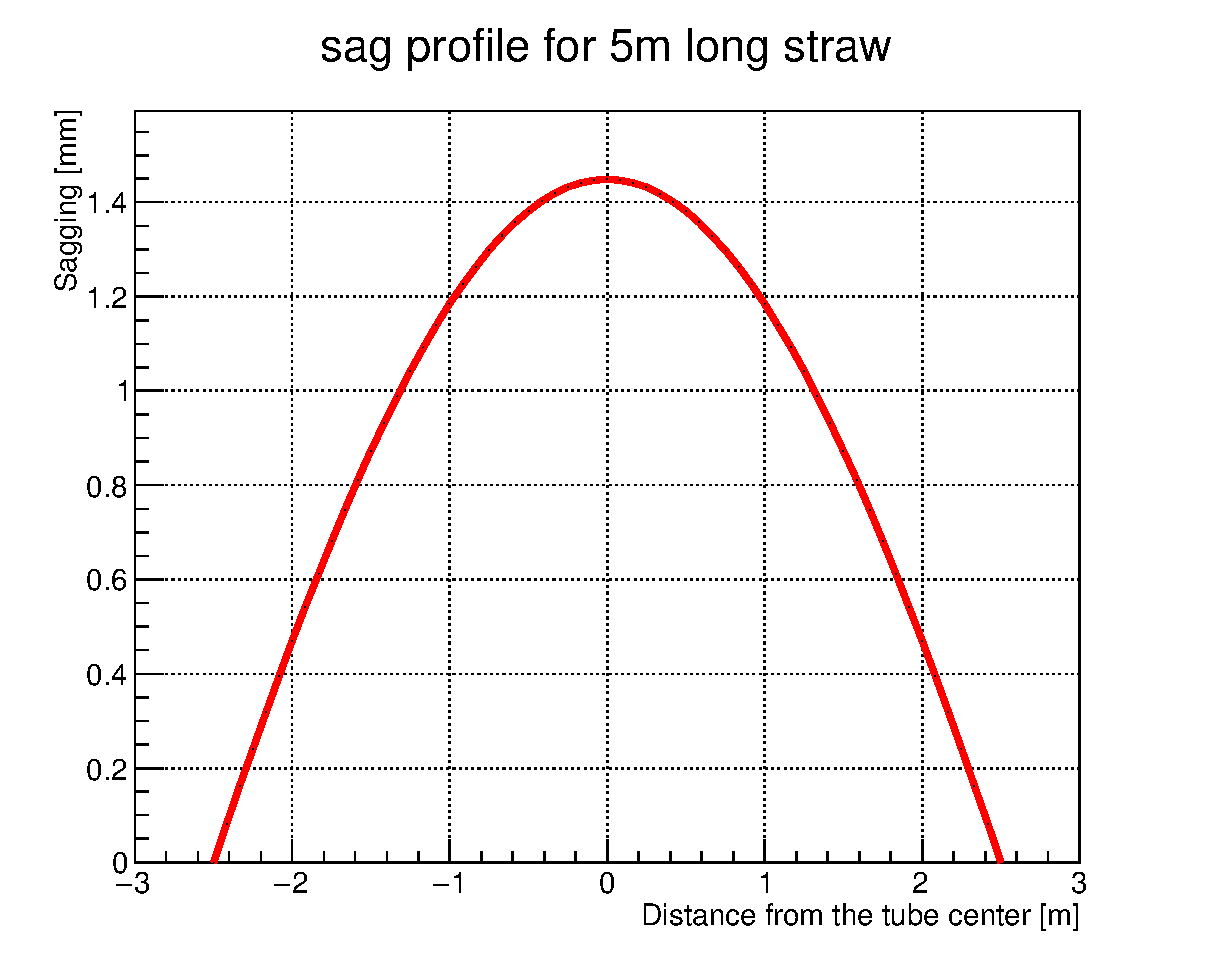
\includegraphics[width=0.7\textwidth]{sagProfileFit.eps}
	\caption{Wire sag profile under electric and gravitation field calculated in GARFIELD. All options for this straw system are described in table~\ref{table:straw_par}.}
	\label{fig:sagProfile}
	\end{figure}	
	
	The calibration of STRAW tube with sagged wire is more difficult by comparison to the mode without sagging. 
	
	Variation of wire tension, wire radius should be taken into account as high affect factor for sag value.
	
	\section{Sag estimation}
	\label{sec:sagEstimation}
	In this section we have to find out method for assessing sagging. This is key step that makes track reconstruction procedure possible.
	
	At first we have to think on data we can use for such kind of calculations. We can extract much useful information  from drift time distribution.
	
	The wire sags under electric and gravitation force. Therefore the sag value differs along the tube (Fig.\ref{fig:sagProfile}). But we can separate collected data for different position along the tube. STRAW tube detector consists of several parallel layers of tubes at some angle to each other. So we can easily fix longitudinal position (along the tube) for tracks that cross several crossed tubes (at least two). Collimation is also possible via scintillator triggering before and after STRAW tube.
	
	Lets say we can install our STRAW tube into homogeneous particle flow and save drift time distribution for some narrow section of the tube. These distributions are different from each other(see example on Fig.\ref{fig:DrftTimeDistr_00_09_comp}). The difference between diagrams increasing with sag difference. So it is good tools for sag calibration.
		
	\begin{figure}[h!]
	\centering
	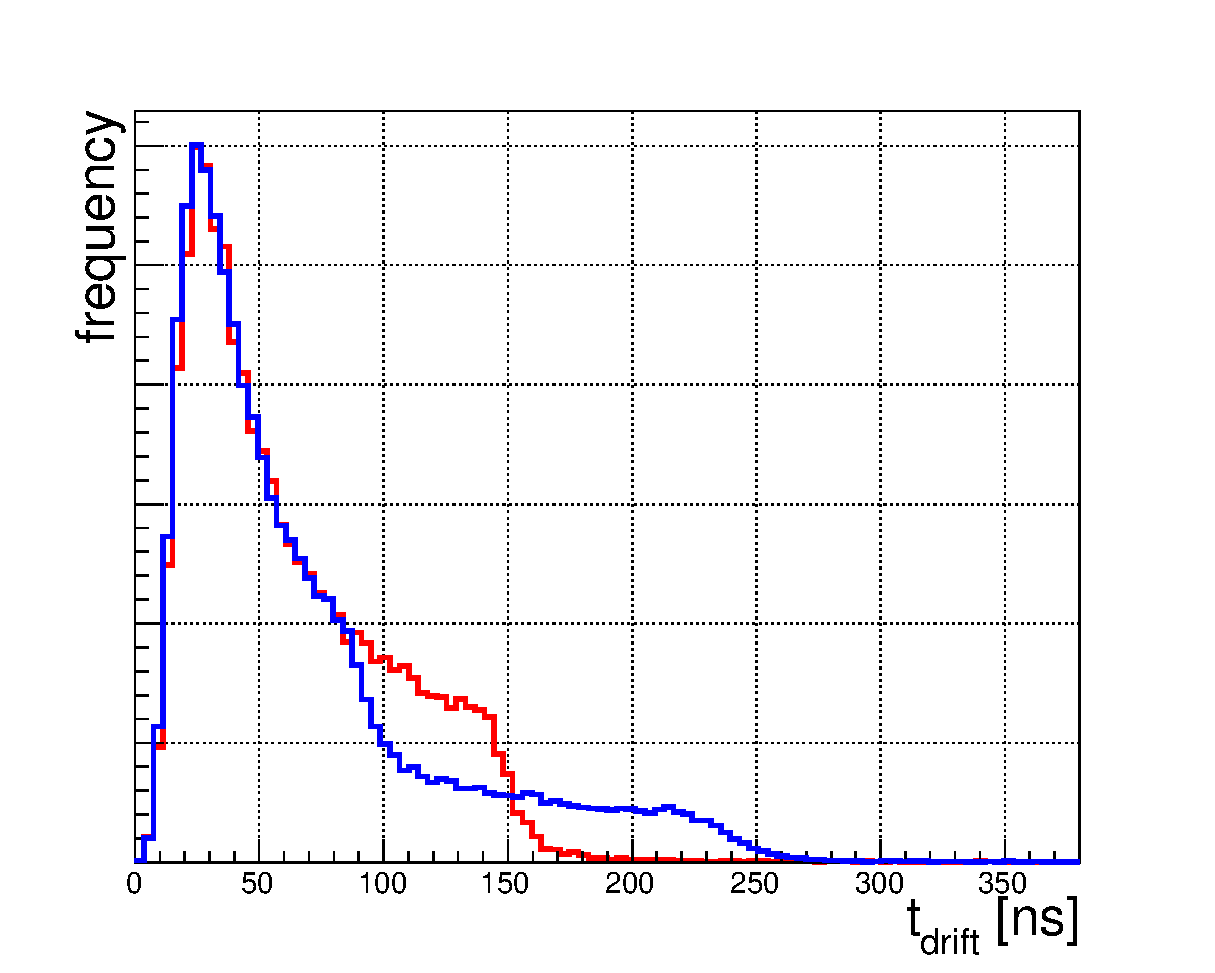
\includegraphics[width=0.8\textwidth]{00_09_driftTimeDistr}
	\caption{Drift time distribution for a homogeneous irradi-
ation with a centered wire (red) and for a wire offset of 0.9 mm (blue).}
	\label{fig:DrftTimeDistr_00_09_comp}	
	\end{figure}
	
	Then we have to bind each drift time distribution with appropriate sag value. This is part of laboratory work when sag profile measurements can be performed via optical method prior to the exposition.
	
	GARFIELD can handle only two-dimensional tasks. So every simulation in this article is plane - as shown in Fig.\ref{fig:electron_ion_track}.
	Distributions on Fig.\ref{fig:DrftTimeDistr_00_09_comp} contains GARFIELD simulations for tube with wire located at certain position (in terms of displacement from tube center).
	
	Lets say we have an equipment for scanning the tube to measure wire sagging profile. After profile measurements we divide our tube into sections.Wire position within separate section should be defined within desired precision
	
	So we need divide our tube on $57$ sections (see Fig.\ref{fig:tube_sectioning}) if maximum of wire offset (at the center of the tube) is equal to $1.45mm$ and desired precision is $50\mu m$.
	
	\begin{equation}
	N_{halftube} = \frac{1.45 mm}{50 \mu m} = 29;
	\label{eq:tube_sectioning}
	\end{equation}
	
	\begin{figure}[h!]
	\centering
	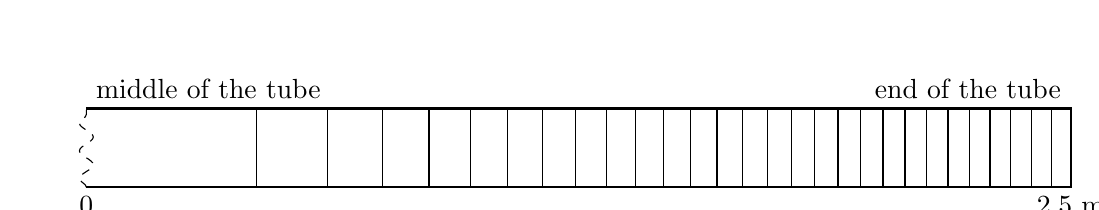
\begin{tikzpicture}[xscale=0.05,yscale=1]
	
	\tikzset{snake it/.style={decorate, decoration=snake}}
	\draw[snake it,dashed] (0,0) -- (0,1);
	
	\draw[thick] (0,0) -- (250,0) -- (250,1) -- (0,1);
	\draw[] (43.2339,0) -- (43.2339,1) -- 
	(61.2704,1) -- (61.2704,0) -- 
	(75.2004,0) -- (75.2004,1) -- 
	(87.0213,1) -- (87.0213,0) -- 
	(97.5056,0) -- (97.5056,1) -- 
	(107.049,1) -- (107.049,0) -- 
	(115.885,0) -- (115.885,1) -- 
	(115.885,1) -- (115.885,0) -- 
	(124.169,0) -- (124.169,1) -- 
	(132.005,1) -- (132.005,0) -- 
	(139.472,0) -- (139.472,1) -- 
	(146.627,1) -- (146.627,0) -- 
	(153.516,0) -- (153.516,1) -- 
	(160.176,1) -- (160.176,0) -- 
	(166.636,0) -- (166.636,1) -- 
	(172.921,1) -- (172.921,0) -- 
	(179.05,0) -- (179.05,1) -- 
	(185.043,1) -- (185.043,0) -- 
	(190.913,0) -- (190.913,1) -- 
	(196.674,1) -- (196.674,0) -- 
	(202.338,0) -- (202.338,1) -- 
	(207.915,1) -- (207.915,0) -- 
	(213.414,0) -- (213.414,1) -- 
	(218.844,1) -- (218.844,0) -- 
	(224.212,0) -- (224.212,1) -- 
	(229.527,1) -- (229.527,0) -- 
	(234.793,0) -- (234.793,1) -- 
	(240.018,1) -- (240.018,0) -- 
	(245.207,0) -- (245.207,1);
	
	\node[below] at (0,0) {0};
	\node[below] at (250,0) {2.5 m};
	\node[above right] at (0,1) {middle of the tube};
	\node[above left] at (250,1) {end of the tube};
	
	\end{tikzpicture} 
	\caption{Tube sectioning. Sag value at the tube center is $1.45mm$. Difference of wire sag value from section to section is $50\mu m$}
	\label{fig:tube_sectioning}
	\end{figure}
	
	Then we need an exposition of sufficient number of events for every of sections(at least 50k events). There can be troubles time of exposition time because square of sections at the end of the tube is quite small. So the time of exposition of distant sections will be inversely much longer.
	
	The next step is to find dependence of dt-distribution shape with wire offset. The point that we can evaluate matching between histograms via $\chi^2$  criteria. As we can see in the figure~\ref{fig:chi2for07} the comparison of  $\chi^2$ has smooth dependence across increasing of wire offset for high statistic histograms.
		
	First steps for sag estimation are:
	\begin{enumerate}
	\item measure wire sag profile via optical method;	
	\item make a sectioning of tube due to wire sag profile;
	\item collect enough amount of events for every of dt-distribution and save this {\it core} distribution for further comparisons.
	\item measure dt-distribution of tube section that is subject of study and and adjacent area.
	\item calculate $\chi^2$ criteria for this current dt-distribution with each of core distribution.
	\item correlate found values of wire displacement relatively to the adjacent sections or by fitting of whole wire profile points.
	\end{enumerate}

	\subsection{Finding most probable value of wire displacement for certain point of the tube}
	
	\subsection{Raw method}
	The simplest method to find $S$ is to equate it to the corresponding value of best matched core DT-histogram.
	
	On the figure \ref{fig:chi_063_5k}  you can see distribution of such kind of reconstruction. Even for 5k events td-distribution in this case the precision can be quite high($\sim 50 \mu m$). This method limited by core DT-diagram stepping.
	
	\begin{figure}[h!]
		\centering
		\subfloat[Series of $\chi^2$ of comparison $0.7 mm$ sag core td-distribution with each each of core histograms. 14 core histograms for sag diapason $0\dots 1.3 mm$ with step of $100\mu m$]{
			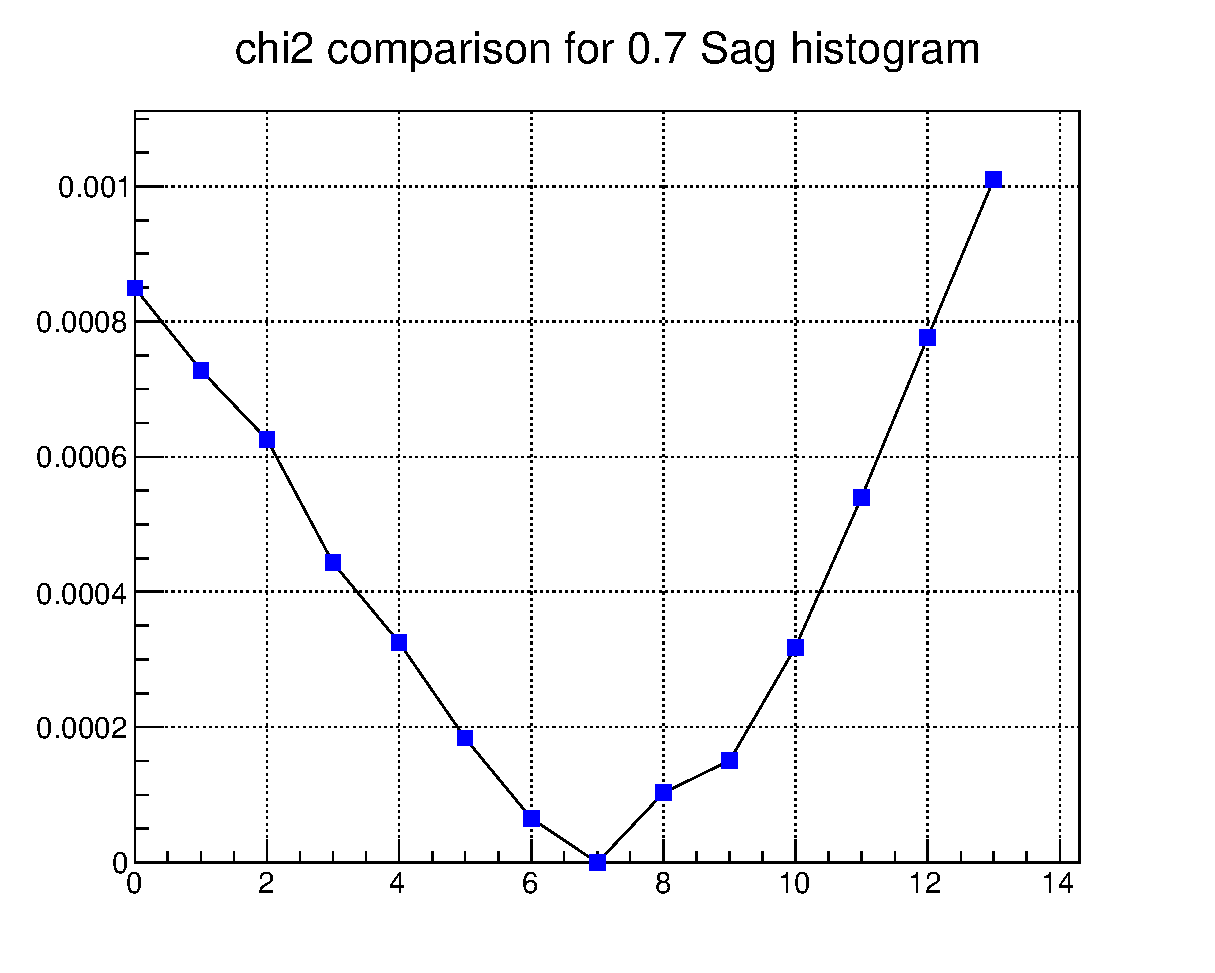
\includegraphics[width=0.45\textwidth]{chi2_07} 
			\label{fig:chi2for07} }%
		\qquad
		\subfloat[ Distribution of wire offset reconstruction from 180 series 5k events each. 50k events for $core$ template histograms. True bias is $0.63 mm$. 1 bin = 0.1 mm.]{
			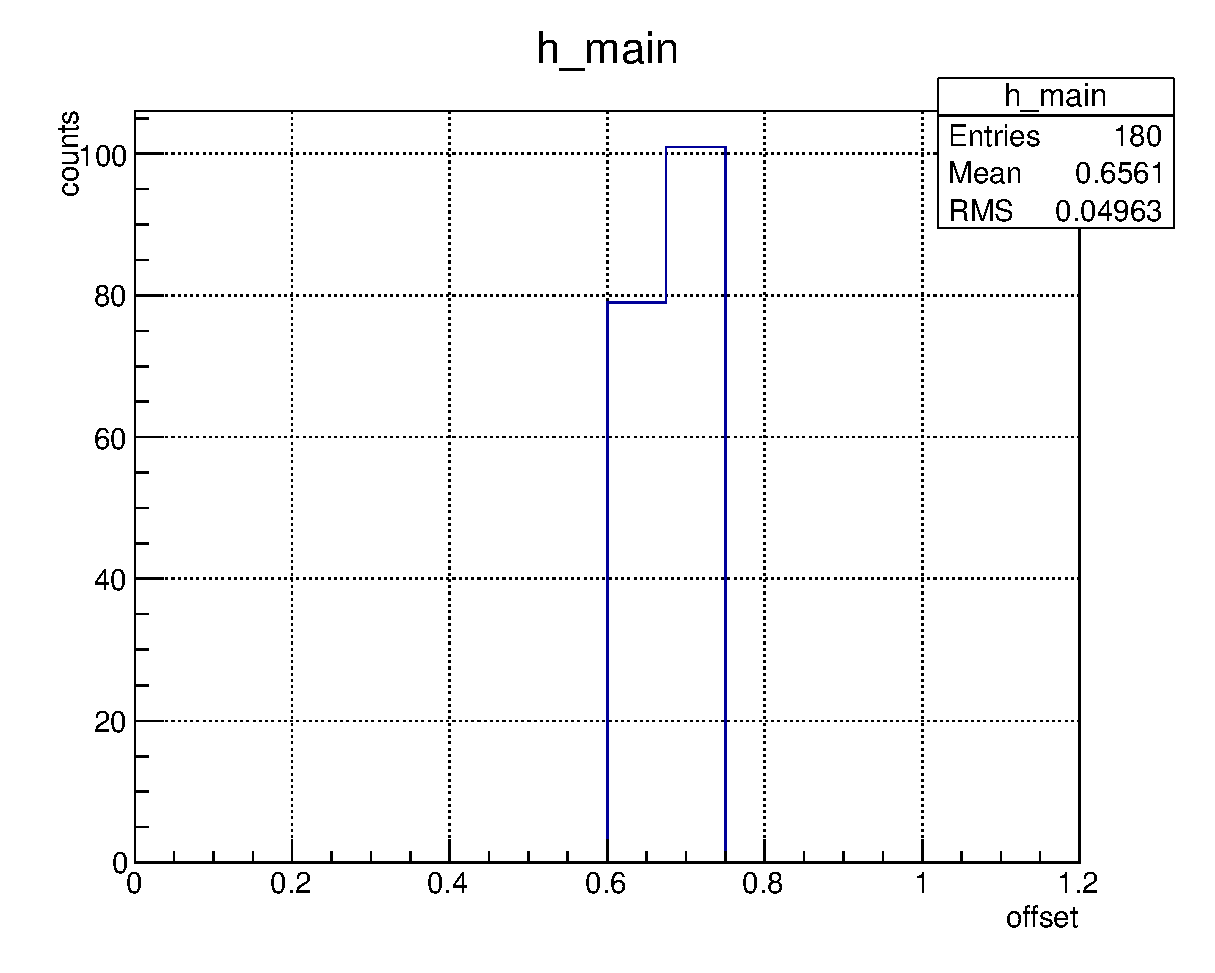
\includegraphics[width=0.45\textwidth]{chi_063_5k} 
			\label{fig:chi_063_5k} }%
		\caption{Wire position(displacement) reconstruction}			
	\end{figure}	
	
%	If we compare dt-distribution for $0.7mm$ displaced wire with each of core dt-distribution you will notice best matching with core histogram for the same wire displacement(see fig see fig~\ref{fig:chi2for07}).
	

	\subsection{"Minimum of $\chi^2$ as linear approximation"}
%	But what is most probable value of wire displacement $S$ in this case? Probably somewhere between them. So can we go in more clever way to reach better result? Probably yes.
	
	If dependence of $\chi^2$ criteria of wire displacement $S$ for near to the true position region is linear(that certainly is not a true, but as first approximation) than we can easily find this intermediate value of wire displacement.
	
	There we proceed in two steps. The first is raw estimation of wire displacement as in above mentioned method.
	
	For the second step we need to know some additional estimations.	The first question is how small can be  $\chi^2$ it our case? Lets fix statistic on 50k events for one DT-distribution. This value should a bit depend for different $S$. But for now lets consider that it is a constant value. From the Fig.\ref{fig:chi2Shelf} you can see distribution of $\chi^2$ from comparison of 20 DT-distribution\footnote{pair comparison give us $C_{20}^2 = \frac{20!}{2!18!}=190$ different combinations}  for $S=0.7mm$. Mean value + RMS of distribution is $ 5.3*10^{-5}$. So if some of the $\chi^2$ is higher than this threshold than we go for second stage.
	
	
	\begin{figure}[h!]
		\centering
		\subfloat[$\chi^2$ distribution of comparison of 20 DT-distributions diagrams each other($C_{20}^2 = 190$ combinations)]{
			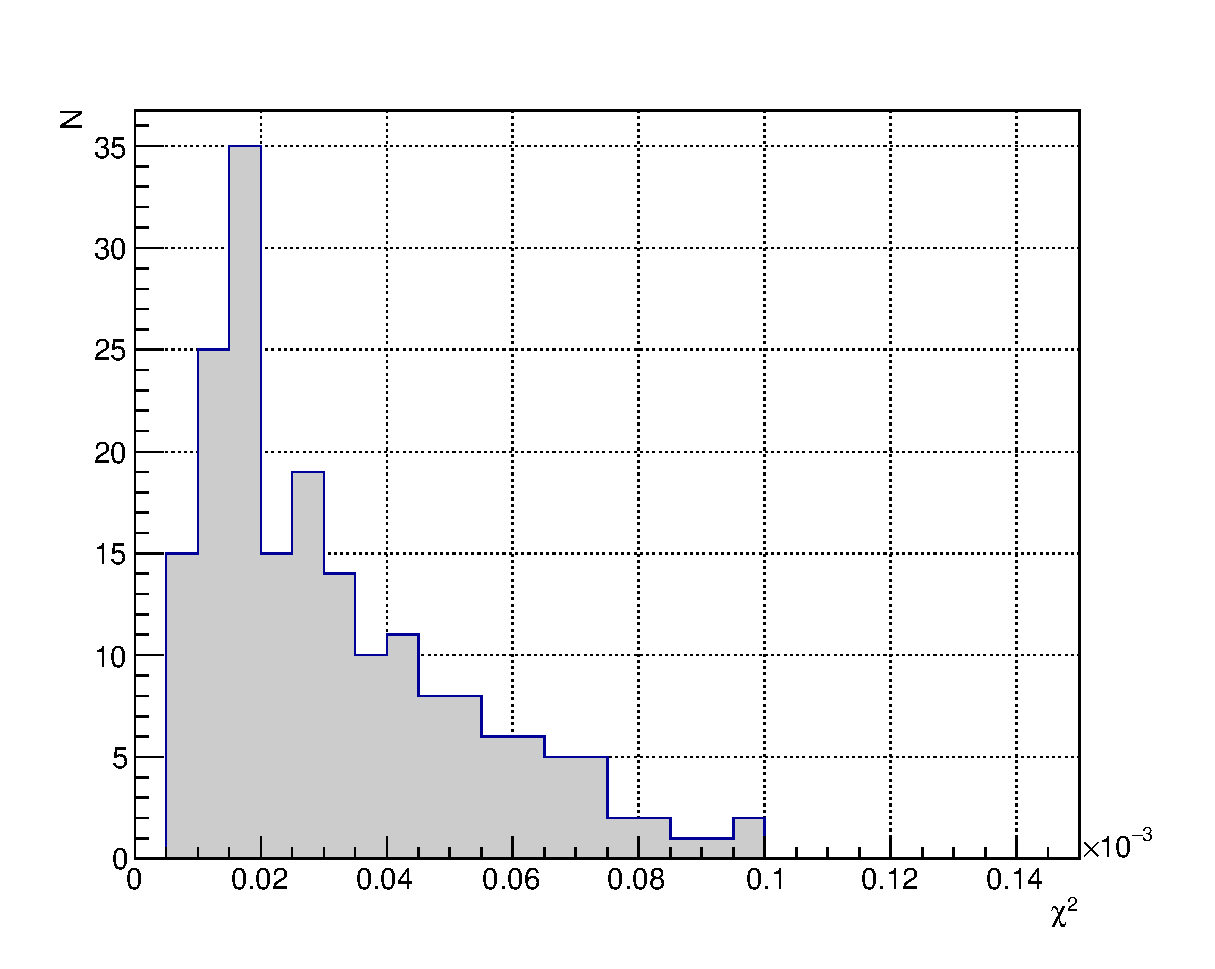
\includegraphics[width=0.45\textwidth]{chi2Shelf} 
			\label{fig:chi2Shelf} }%
		\qquad
		\subfloat[$\chi^2$ distribution of comparison DT-distribution histograms $0.6 mm$ S vs $0.7 mm$ ]{
			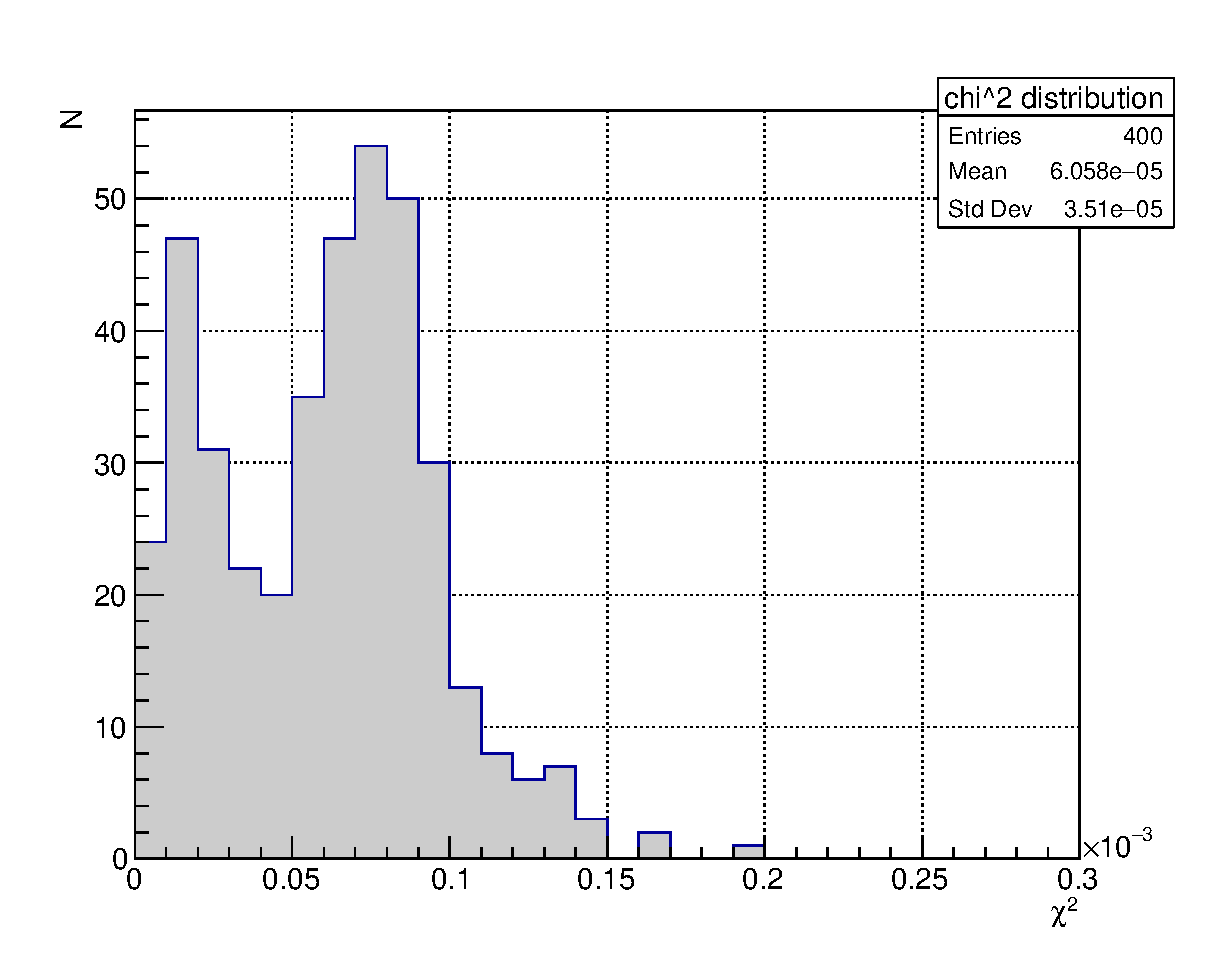
\includegraphics[width=0.45\textwidth]{06_07_chi_stat} 
			\label{fig:06_07_chi_stat} }%
		\caption{Comparison of $\chi^2$ distributions for self-comparison of DT-distribution diagram.} 
	\end{figure}	
	
	On the Fig.\ref{fig:chi_063_5k} you can see distribution of wire sag calculation for 180 histograms with 5k events statistic. Precision in this case  $\sim 50\mu$. The algorithm of sag estimation is pretty simple: wire offset value is equal to the offset  of best matched  $core$ histogram.

	After we know sag value at some points of the tube or every where we can make one awesome collective analysis. The smoothing of wire offset value along the tube will give to us much more precision results.  
	
	From the Fig.\ref{fig:06_07_chi_stat} the distribution of $\chi^2$ for adjacent point have narrower distribution by comparison to "self-comparison" $\chi^2$ distribution. Therefore calculation of $S$ from analyse of consecutive smallest $\chi^2$ values can improve precision.
	Need to say that collective approach to this task also can improve precision of $S$ finding. 
	
	
	\subsection{Practical measurements of DT-distribution}
	
	We need second detector that can measure position of muon that hit STRAW tube. It can be Si strip sensor based detector or detector based on  scintillation with the same destination.
	
	Each kind of detector have it's own advantages and disadvantages. The potential cell unit (strip of pixel) of Si detector will be smaller than in scintilator but also is match expensive. At the current stage we deal with $1cm$ diameter tubes. So scintilator is primal target. But it can shift to the Si sensors if scintilators will not provide satisfied precision.
	
	Preliminary chem of DT-measurements you can see on the picture Fig.\ref{fig:DT-mesure-layout}
	
	\begin{figure}[h!]
	\centering
	\begin{tikzpicture}
	
	\tikzset{snake it/.style={decorate, decoration=snake}}
	
	\draw (-1,0) -- (-1,10);
	\draw ( 1,0) -- ( 1,10);
	\draw (0,0) ellipse (1 and .3);
	\draw (0,10) ellipse (1 and .3);
	
	\draw (-5,0) -- (-6,0);
	\draw (-5,.5) -- (-6,.5);
	\draw (-5,1) -- (-6,1);
	\draw (-5,1.5) -- (-6,1.5);
	\draw (-5,2) -- (-6,2);
	\draw (-5,2.5) -- (-6,2.5);
	\draw (-5,3) -- (-6,3);
	\draw (-5,3.5) -- (-6,3.5);
	\draw (-5,4) -- (-6,4);
	\draw (-5,4.5) -- (-6,4.5);
	\draw (-5,5) -- (-6,5);
	\draw (-5,5.5) -- (-6,5.5);
	\draw (-5,6) -- (-6,6);
	\draw (-5,6.5) -- (-6,6.5);
	\draw (-5,7) -- (-6,7);
	\draw (-5,7.5) -- (-6,7.5);
	\draw (-5,8) -- (-6,8);
	\draw (-5,8.5) -- (-6,8.5);
	\draw (-5,9) -- (-6,9);
	\draw (-5,9.5) -- (-6,9.5);
	\draw (-5,10) -- (-6,10);
	
	\draw (-5,0) -- (-5,10);
	\draw (-6,0) -- (-6,10);

	\draw (5,0) -- (6,0);
	\draw (5,.5) -- (6,.5);
	\draw (5,1) -- (6,1);
	\draw (5,1.5) -- (6,1.5);
	\draw (5,2) -- (6,2);
	\draw (5,2.5) -- (6,2.5);
	\draw (5,3) -- (6,3);
	\draw (5,3.5) -- (6,3.5);
	\draw (5,4) -- (6,4);
	\draw (5,4.5) -- (6,4.5);
	\draw (5,5) -- (6,5);
	\draw (5,5.5) -- (6,5.5);
	\draw (5,6) -- (6,6);
	\draw (5,6.5) -- (6,6.5);
	\draw (5,7) -- (6,7);
	\draw (5,7.5) -- (6,7.5);
	\draw (5,8) -- (6,8);
	\draw (5,8.5) -- (6,8.5);
	\draw (5,9) -- (6,9);
	\draw (5,9.5) -- (6,9.5);
	\draw (5,10) -- (6,10);
	
	\draw (5,0) -- (5,10);
	\draw (6,0) -- (6,10);
	
	\node [below] at (5,0) {detector 2};
	\node [below] at (-5,0) {detector 1};
	\node [] at (0,-1) {STRAW tube};


	\draw[ultra thick,->] (-10,7.5) -- (-6.5,7.5);
	\draw[ultra thick,->] (-10,7) -- (-6.5,7);
	\draw[ultra thick,->] (-10,6.5) -- (-6.5,6.5);
	\draw[ultra thick,->] (-10,6) -- (-6.5,6);
	\draw[ultra thick,->] (-10,5.5) -- (-6.5,5.5);
	\draw[ultra thick,->] (-10,5) -- (-6.5,5);
	
	\node at (-8,8) {muon flow};
	
	\draw[thick] (-8,3) ellipse (0.3 and 0.3);
	
	\draw[thick] (-8-0.2, 3-0.2) --(-8 +0.2, 3+0.2);
	\draw[thick] (-8-0.2, 3+0.2) --(-8 +0.2, 3-0.2);

	\node[] at (-8.5,3) {$\vec{g}$};
		
	\end{tikzpicture} 
	\caption{principal layout of measurement of core DT-distribution histogram}
	\label{fig:DT-mesure-layout}
	\end{figure}	
	
	In this method detector before tube (D1) and detector placed after the tube(D2) in total should provide sufficient precision for track reconstruction to be able distinguish tracks for different section of the tube (approximately as shown on the Fig. \ref{fig:tube_sectioning}). Muon flow should be homogeneous and so D1 and D2 also should cover full acceptance of the tube.
	
	The profile of the wire sagging can be measured by optical method. Walls of the tube is very thin, so it can be simplest way to get sag profile.
	
	
	\section{Track reconstruction}
	
	The time between the track hit time stamp and the signal rising edge is a measure of {\it drift time} of these electrons. The relation between the   {\it drift time} and  the distance from the track to the center of the tube(wire while no sag for centered wire) is called {\it drift time - distance} relation or {\it tr-relation}.
	
	The drift time $t$ is a function of track position (relative to the wire) and electric field along the drift trajectory.
	
	Assumed that the working  position  for straws will be parallel to the particle bunch, and  acceptance of particle spreading will not be significantly big. So tracks will be collinear each other within every separate  STRAW tube unit.
	
	Summing the above mentioned we have one dimension task -- reconstruct tracks on vertical axis\footnote{An example of single track reconstruction which explains the approximate procedure of reconstruction you can see on Fig.\ref{fig:track_reconstruction}}	(see examples of outcome tr-distribution $t = t(r,s=0)$ in Fig.\ref{fig:t_r_distr_00} and Fig.\ref{fig:tr_distr_15})  even the wire sagging. Sagging will be always down thanks to gravitation force $\vec{g}$.
	
	\begin{figure}[h!]
		\centering
		\subfloat[wire at the center]{
			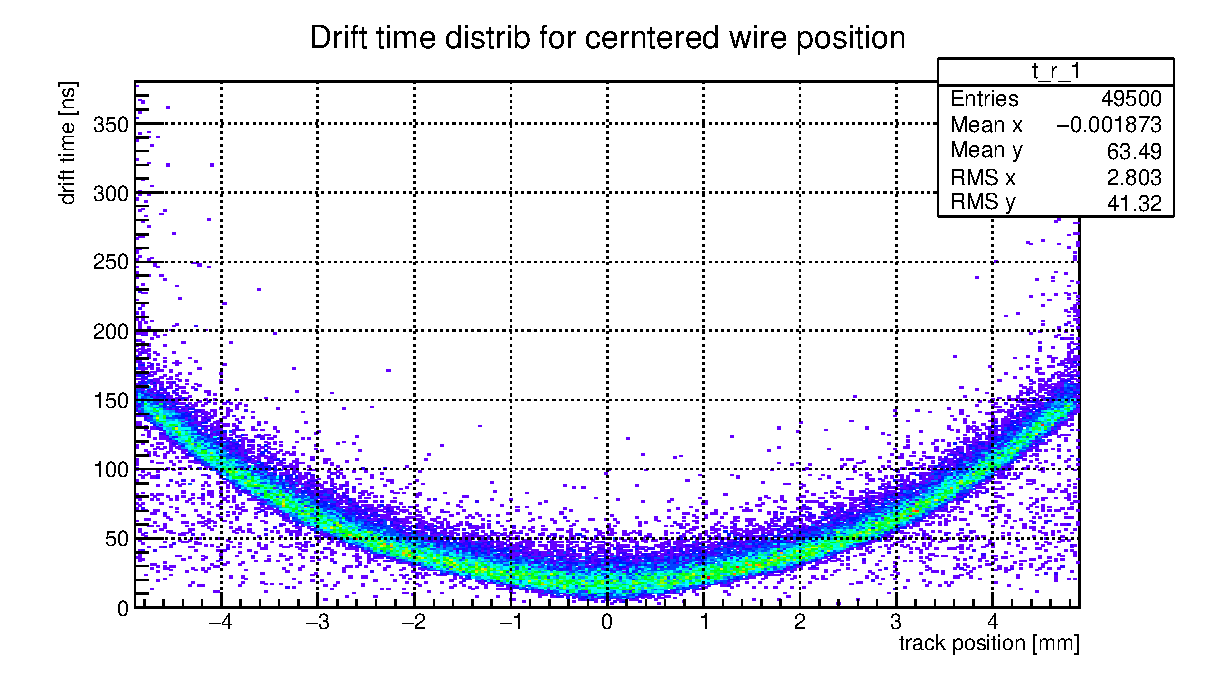
\includegraphics[width=0.45\textwidth]{t_r_distr_00} 
			\label{fig:t_r_distr_00} }%
		\qquad
		\subfloat[$1.5mm$  offset]{
			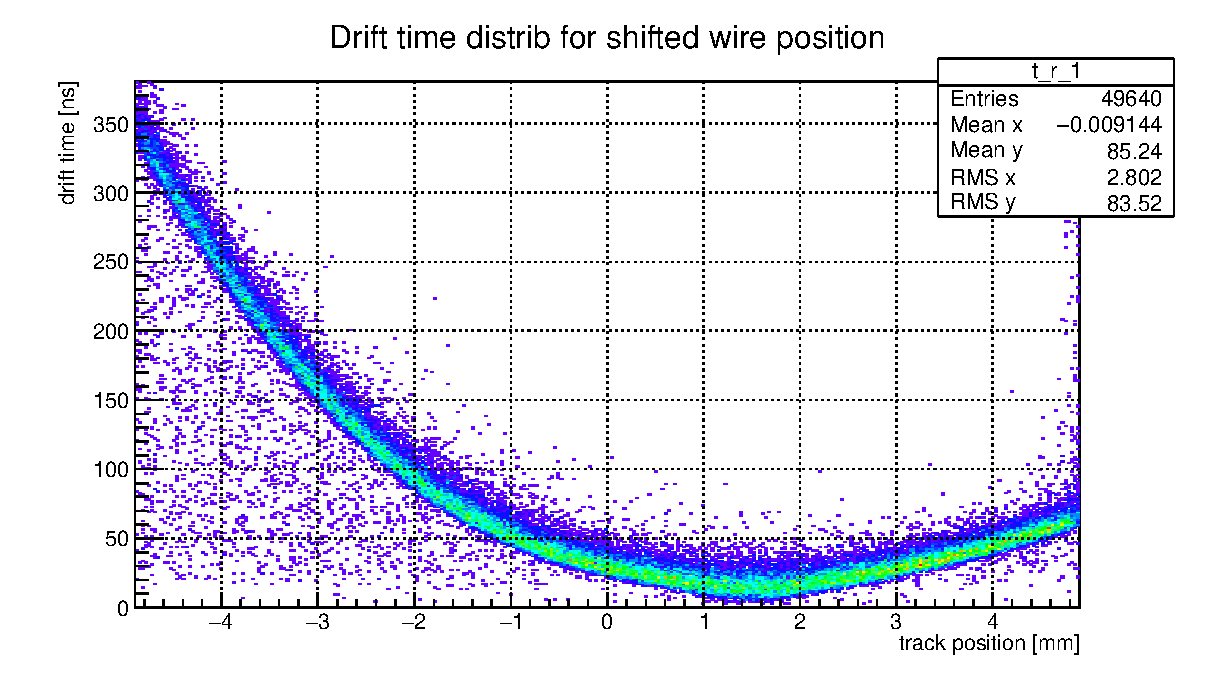
\includegraphics[width=0.45\textwidth]{tr_distr_15} 
			\label{fig:tr_distr_15} }%
		\caption{Distribution of drift time $t_{drift}$ as function of track position $r_{track}$ relatively to the tube center}			
	\end{figure}	
	
	The rt-relation is differ along the tube because different wire position $s$. Thus we have for the drift time 
	\begin{equation}
	t_{drift} = t_{drift}(r_{track},s)
	\end{equation}
	
	The idea to STRAW tube is to find the inverse dependence
	\begin{equation}
		r_{track} = r_{track}(t_{drift},s)
	\end{equation}
	
	From the section "Sag estimation" we can find sag profile for straw. Therefore the rt-calibration becomes 1 dimension less:
	\begin{equation}
		r = r(t,s=const)
	\end{equation}
	
	
	\subsection{How drift time resolution depend on wire offset?}
	
	Distorting of electric field inside the tube invoked by wire displacement from the center position will make an effect on drift time. Here we are going to estimate magnitude of drift time change.
	
	As was noted above we make a binning  for our data along the $r_{track}$(fig. \ref{fig:t_r_distr_00}, \ref{fig:tr_distr_15}). The resolution at every bin  is RMS of every bit digram (fig.\ref{fig:driftTimeResolutionEvo}).
	
	\begin{figure}[h!]
		\centering
		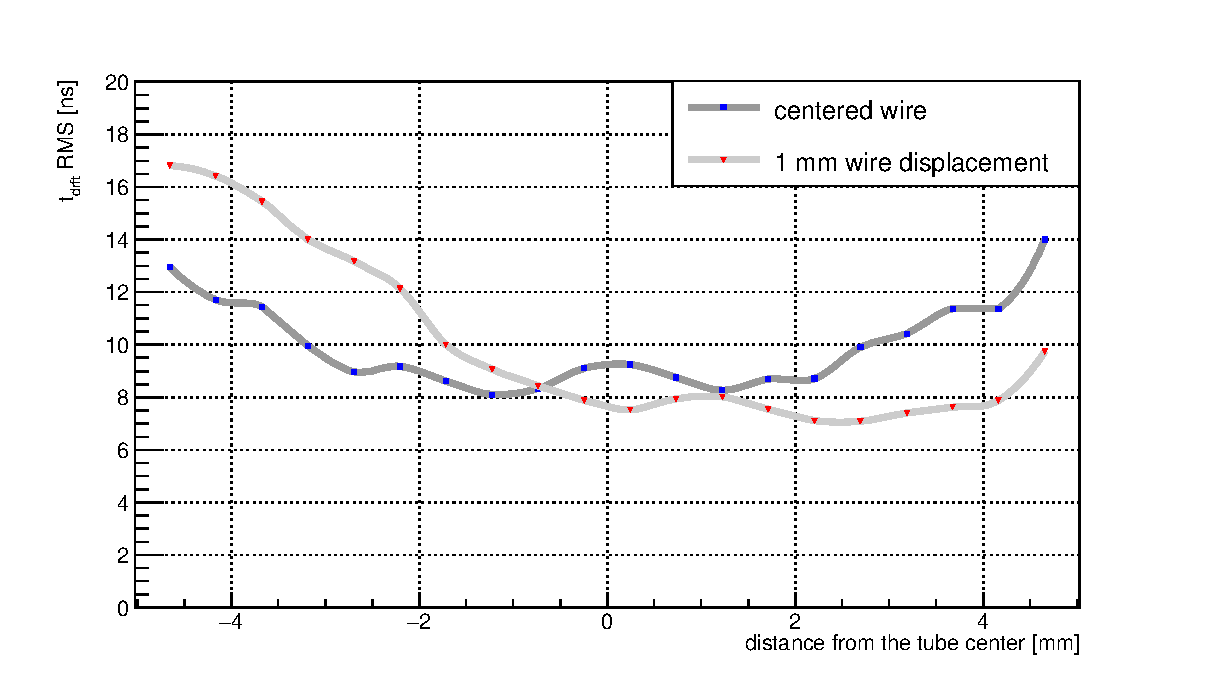
\includegraphics[width=0.9\textwidth]{DTimeRMS2}
		\label{fig:driftTimeResolutionEvo}
		\caption{Resolution of drift time as a function of distance from the wire.}
	\end{figure}
	
	We are dealing with probabilistic  nature of clustering that spread rt-relation from thin line. The leakage noise is also present in calculation but the effect of it i snot very high(especially in this calculation).
	
	Every plot of output current (see fig. \ref{fig:signal_example}) consist of 1000 equidistant frames. The threshold is set to $5\sigma$ of noise. Leakage nose make effect on drift time measurements in case its amplitude becomes higher that threshold value in range from $t=0$ to $t= t_{drift}$. At five-sigma there is only one chance in nearly two million that a random fluctuation would yield the result. The drift time for tracks close to the tube edge can be up to $150 ns$ and $300 ns$ in case wire displaced. The probability to meet noise above threshold value is less than $0.02\%$.
	
	Another source of noise points on tr-distribution comes from $\delta$-electrons that cause secondary ionisation in tube volume. The impact do only those electrons which are emitted in the direction of the wire(see example on fig.\ref{fig:deltaElectron}).
	
	\begin{figure}[h!]
		\centering
		\subfloat[$\delta$-electron affects on drift time]{
			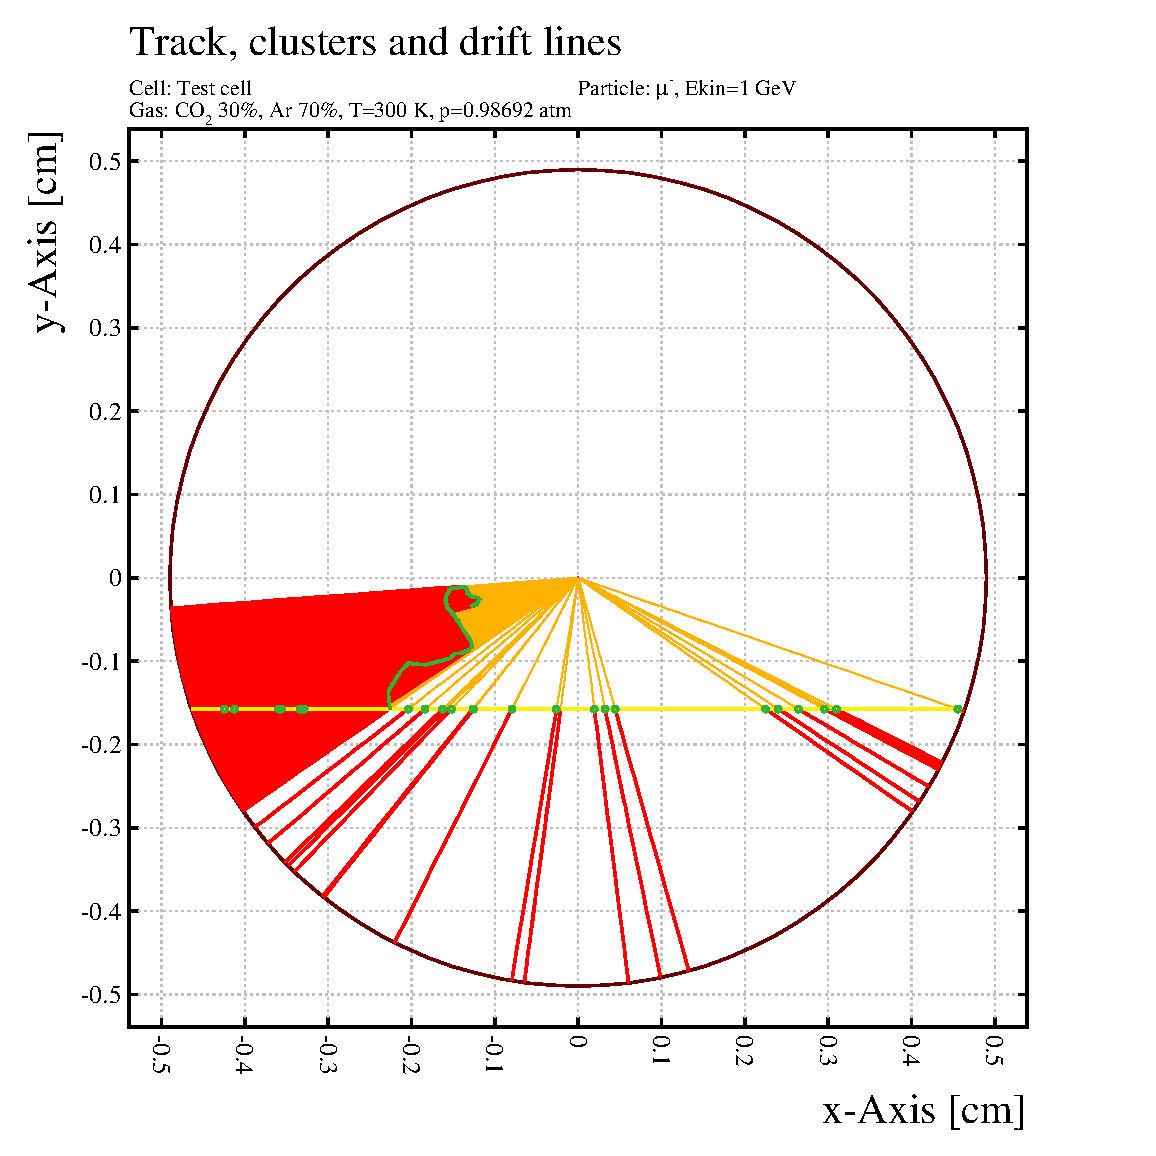
\includegraphics[width=0.45\textwidth]{deltaElectron} 
			\label{fig:deltaElectron} }%
		\qquad
		\subfloat[$\delta$-electron that moves away from the wire has no affect on drift time]{
			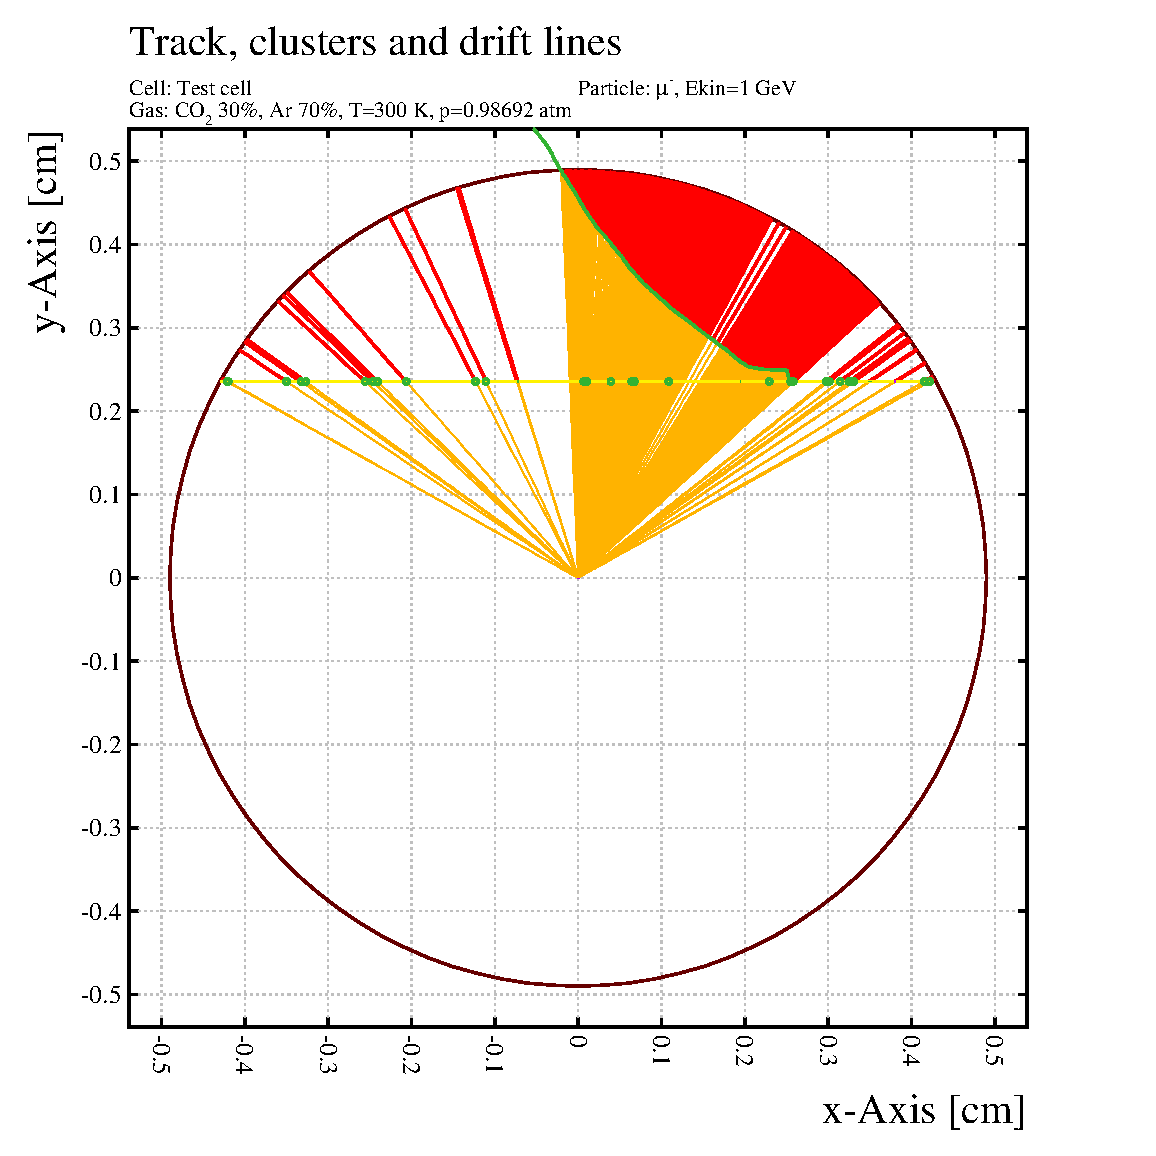
\includegraphics[width=0.45\textwidth]{deltaElectronNoEffect} 
			\label{fig:deltaElectronNoEffect} }%
		\caption{Garfield simulation with $\delta$-electron presence. Red lines - ion trajectory, yellow - electrons. Trajectory of $\delta$-electron marked by green curve line.}			
	\end{figure}	
	
	The number of events out of TR-ralation because of $\delta$-electrons is quite small. Especially percentage of events where $\delta$-electrons make effect on drift time is less that $1\%$ of total number of events  in GARFIELD simulations. 
	
	Tube wall is very thin but particle still can cause $\delta$-electrons when crossing it. GEANT4 studies show that such kind effect also presents in interaction of muon with tube volume, and percentage of events with $\delta$-electron that affect drift time even less that $0.2\%$.
	
	\subsection{Finding of rt-relation}
	
	The rt-relation depict relation between drift time and track position. The idea is to find the best fit of give data to achieve higher resolution and avoid systematic errors.
	
	The problem that we have to minimize influence of noise while fit. One suppose that the noise have approximately homogeneous distribution of points that locates below the main line of distribution. Consequently we can filter it by fitting only points from regions with local point density higher that some threshold value. Another way is to make a binning our distribution along the track position and fit every 1-D histogram by Gaussian. The fit points of Gaussian mean values by fit function.    
	
	Nevertheless our data contain very small amount of "non-track" points.
	
	TR-relation is asymmetry relatively to the $r=0$ almost in all cases except wire in the center of the tube. Therefore we have to calibrate for every of branches. It means we need to find two track positions for every of drift time value and reject one of them in further data processing stages.
	
	In previous section we found way to measure wire sag profile. So we can use this trick in present stage for separating data into ``right'' and ``left'' branch. Every of branches we will calibrate separately.
	
	Lets suppose we can fit every of tr-diagram by pair of analytic fit function (\ref{eq:trRelation}):
	\begin{equation}
	t(r_{track}) = e^{a_0 + a_1r_{track}}
	\label{eq:trRelation}
	\end{equation}
	
	\begin{figure}[h!]
	\centering
	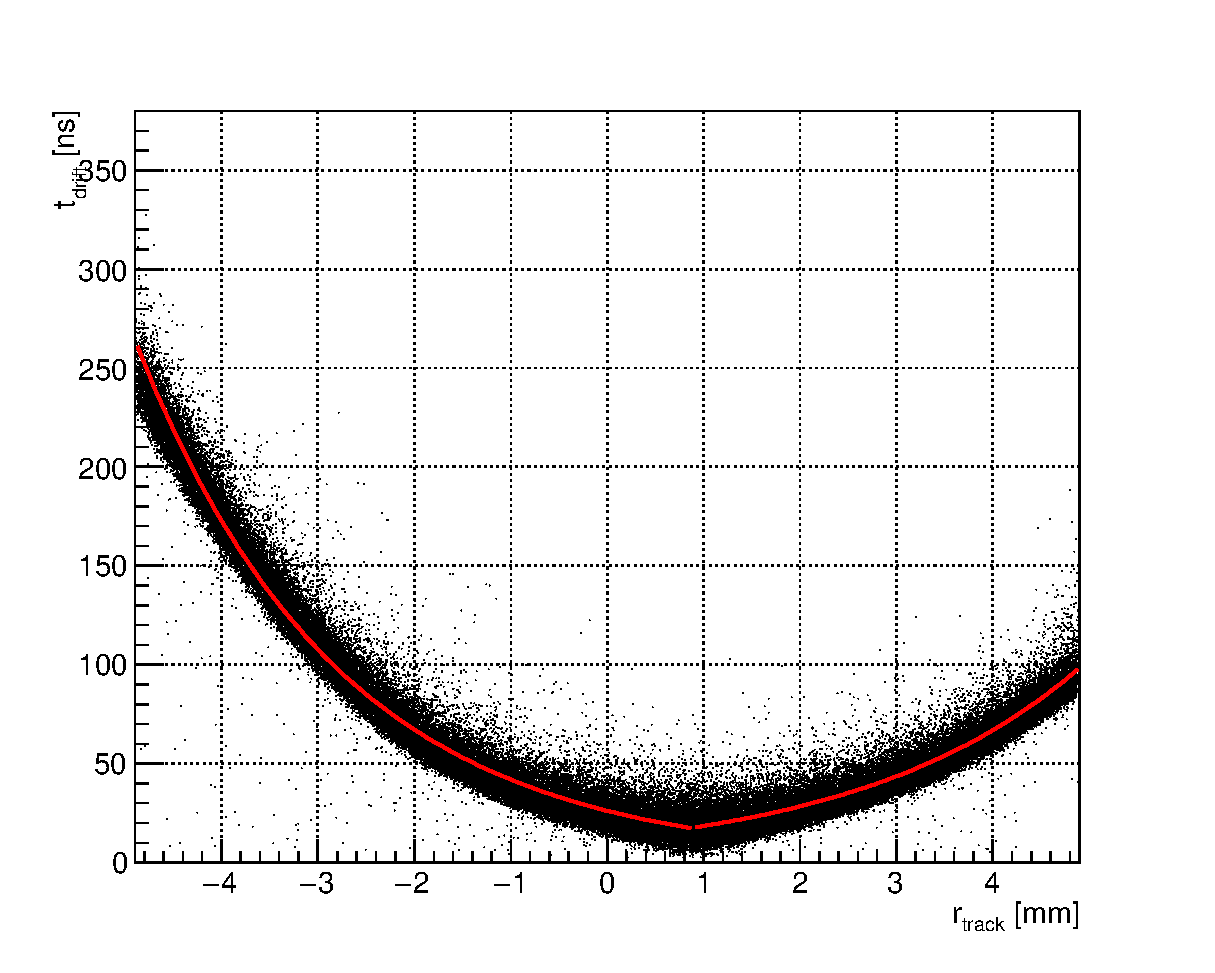
\includegraphics[width=0.7\textwidth]{TRrelation_09_points}
	\label{fig:TRrelation09points}
	\caption{TR-relation fitting for $0.9 mm$ wire offset value}
	\end{figure}
	
	If the figure \ref{fig:TRrelation09points} you can see tr-relation. Fitting is not perfect because of using simple fit function template (\ref{eq:trRelation}). But we will use reverse to the (\ref{eq:trRelation}) relation, because we have to find $r_{track}$ from known $t_{drift}$. We can do it be because the aim of this studies is not a precision calibration but global evaluation affect of wire sagging into total result.
	
	As you can see in the figure \ref{fig:TRrelation09points} red fit line does not cover whole drift time spectre. So events with drift time less than covered range(less than $\sim20 ns$) counts as track through the wire:
	\begin{equation}
	r_{track}(t_{drift} < t_{min}) = r_{wire~pos}
	\end{equation}
	where $t_{min} = min (t_{drift}(r_{track}))$, $r_{track} = \overline{(-r_{tube},r_{tube})}$. Respectively tracks with drift time higher than maximum of fit function range artificially counts as tracks with near tangents to the tube position $r_{track} = \pm r_{tube}$  (because efficiency decreases near the tube wall down to $20\%$).
	
	\subsection{Track reconstruction precision}
	
	Obviously precision is head factor when during we decide design of detector.
	
	The STRAW tube tracker should be as light as possible to avoid multiple scattering on structural components of detector. But design should be changed within reason if precision suffers from this\footnote{Especially design with no sagging works well for experiment NA62 \cite{}. But they have more than 2 times shorter  straw when tube have insert in the middle of the tube. So sagging becomes negligible in this case.}.
	
	How precision of track reconstruction depends on wire position(wire displacement)?
	
	\begin{figure}[h!]
		\centering
		\subfloat[reconstructed track position $r_{rec}$ as function of true track position $r_{track}$]{
			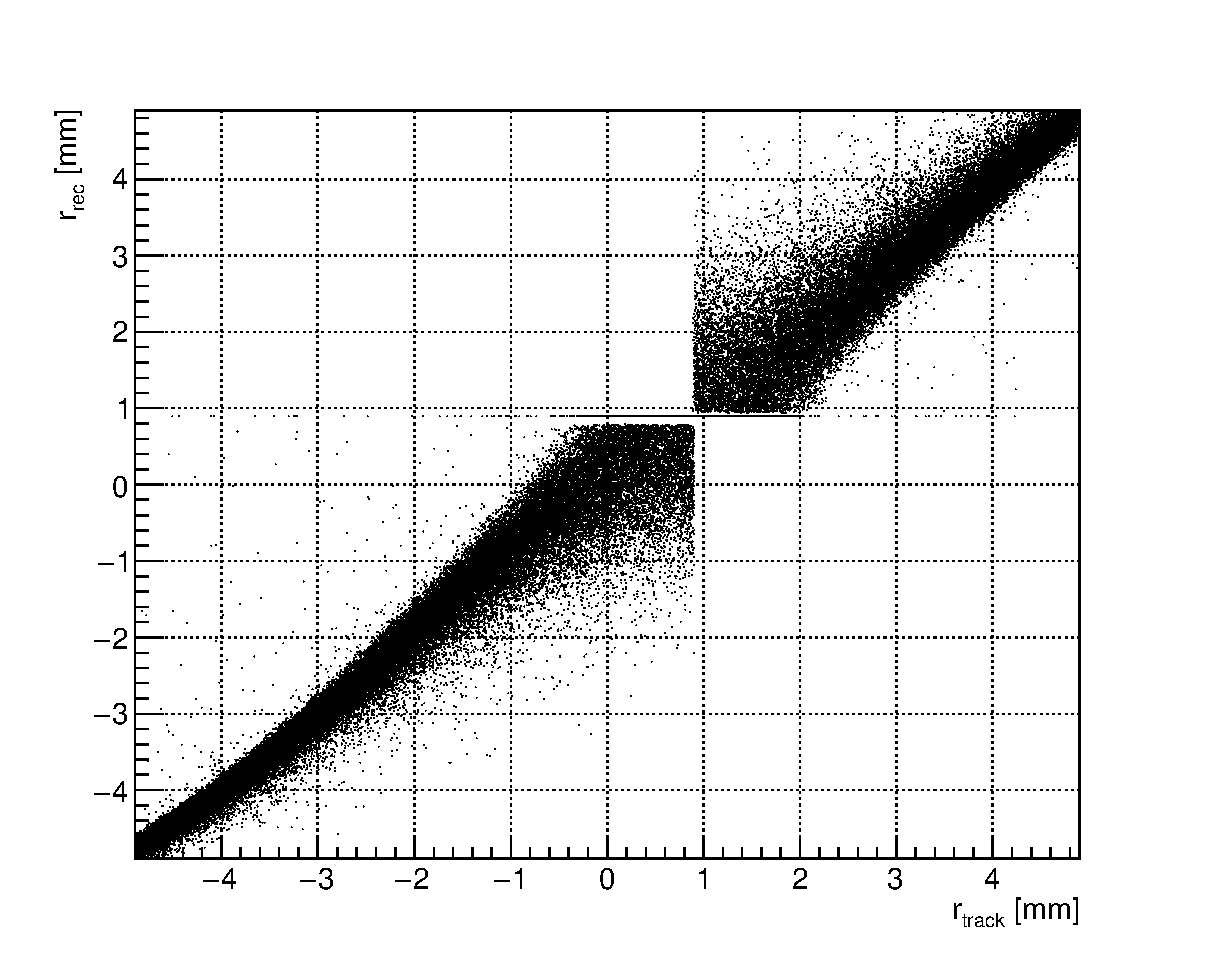
\includegraphics[width=0.4\textwidth]{reconstructed_points} 
			\label{fig:reconstructed_points} }%
		\qquad
		\subfloat[$r_{track} - r_{reconstructed}$ as function of $r_{track}$]{
			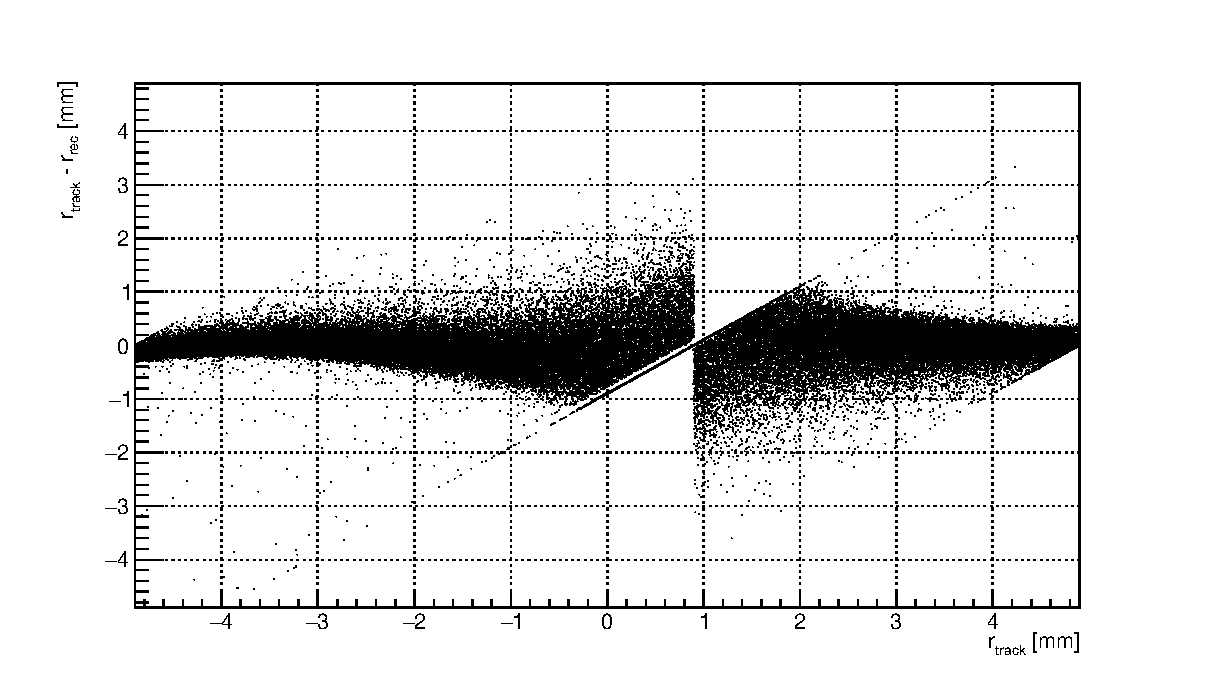
\includegraphics[width=0.5\textwidth]{diffRecTrue09_points} 
			\label{fig:diffRecTrue09_points} }%
		\caption{Distributions of matching of track position to their reconstructed value.}
	\end{figure}
	
	\begin{figure}[h!]
	\centering
	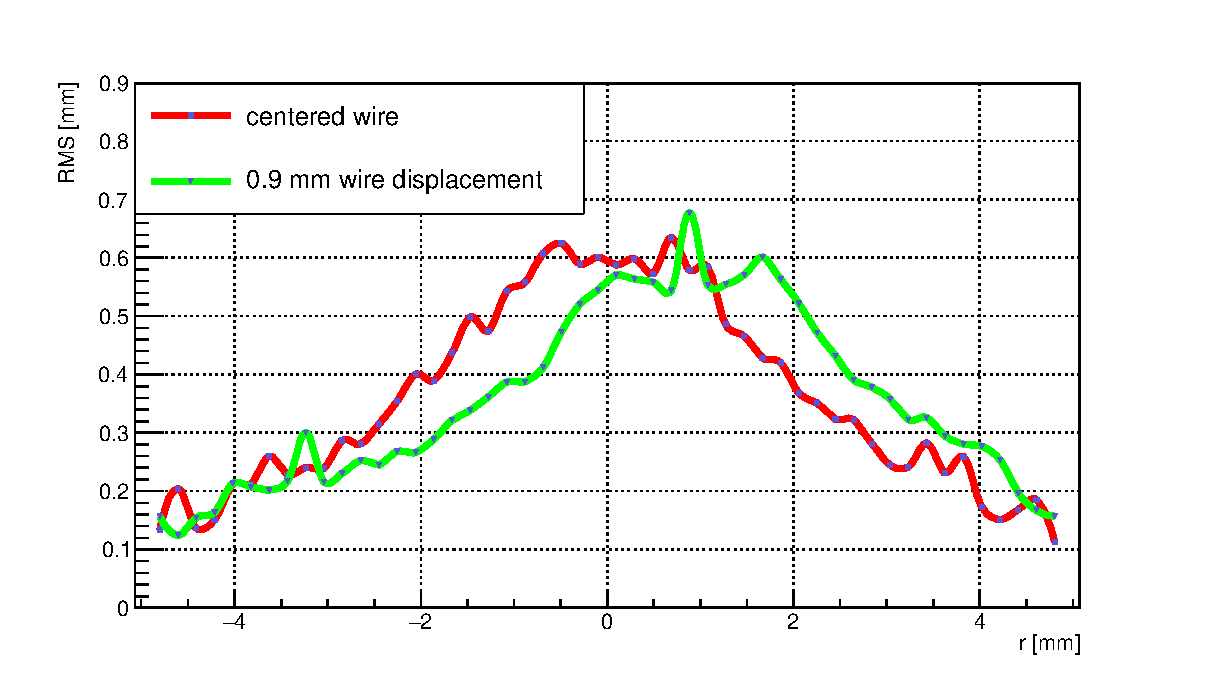
\includegraphics[width=0.9\textwidth]{precisionCompare_0_9}
	\label{fig:precisionCompare09}
	\caption{Comparison of track reconstruction precision for two wire position. Value of precision at every point means RMS of data sample near corresponding track position $r$. Red line corresponds to the centered wire position, green line -- to the $0.9 mm$ sagged wire  position.}
	\end{figure}
	
	As you can see on figure \ref{fig:precisionCompare09} there are no significant difference of track reconstruction precision between two mode of wire location despite of the increasing drift time for displaced wire position(with almost factor of two).	 The highest resolution($\sim 0.1 mm$) near the tube wall and worst value $\sim0.6mm$ is near the wire because the clustering effect. Higher gas pressure should resolve this problem.	
	
	\section{Measurements} 
	\label{sec:Mesurements}	
	
	We made measurements of some important drift tube parameters. We had tube of $\sim 50cm$ length. But despite of short tube length we made measurements where the length of the tube is not important.
	
	The tube was manufactured in Dubna town(Russian Federation) and was placed into the appropriate  mechanic equipment which include tube fixing, channels for supply of gas mixture, connector for grounding to the tube walls and connector for High Voltage (HV) supply.
	
	The whole system is not compact, therefore we could not avoid the parasitic capacities. Now we will not go into details about it, as we have nothing to compare with because the system is non-separable.

	The scheme of gas supply, circulation and control in the tube is shown in the Fig.\ref{fig:gasFlowScheme}.
	
	\begin{figure}[!h]
	\centering
	\begin{tikzpicture}
		\node[inner sep=0pt] (ballon) at (1.8,0)
			{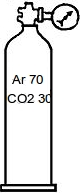
\includegraphics[width=.15\textwidth]{ballon.jpg}};
%		\draw[very thick] (1.2,2.5) -- (2,2.5);
%		\draw[very thick] (2.5,2.5) circle [radius=0.5];
%		\node[] at (2.5,2.5) {$\nearrow$};
		\draw[very thick] (3,2.5) -- (5.5,2.5);
		\draw[thick](4-.2,3) -- (4+.2,2) -- (4-.2,2) -- (4+.2,3) -- (4-.2,3);
		\node[below] at (4,2) {flowmeter1\footnote{flowmeter $V\ddot{o}gtim~V100$}};
		
		\draw (5.6,2.5) ellipse (.1 and .2);
		\draw (5.6,2.7)-- (8,2.7);
		\draw (8,2.5) ellipse (.1 and .2);
		\draw (8,2.3) -- (5.6,2.3);
		\node [below] at (6.6,2.3) {tube};
		
		\draw[very thick] (8,2.5) -- (11,2.5);
		
		\draw[thick](10-.2,3)--(10+.2,2)--(10-.2,2)--(10+.2,3)--(10-.2,3);
		\node[below] at (10,2) {flowmeter2};
		
		\draw[very thick] (8.5,2.5)--(8.5,.5);
		
		\draw(8.5,0) circle [radius=0.5];
		\node at (8.5,0) {P};
		\node[left] at (8,0) {pressuremeter};
		
		\draw[very thick] (11,2.5) -- (11,.5);
		\draw(11,0) circle [radius=0.5];
		\node at (11,0) {B};
		\node[below] at (11,-.5) {Bubbler};
		
		\draw[very thick] (11.5,0) -- (12.5,0) -- (12.5,1);
		\node[above] at (12.5,1) {atmosphere};
	\end{tikzpicture}
	\caption{Gas circulation scheme and circuit of connection of flow control through the drift tube}
	\label{fig:gasFlowScheme}
	\end{figure}		
	
	The electric scheme of the drift tube connection is shown in the Fig.\ref{fig:electricCircuit}.
	
%	Електронна схема підключення дрейфової трубки зображена на рис. \ref{fig:electricCircuit}.
	
	\tikzset{circuit declare symbol = ammeter}
	\tikzset{set ammeter graphic ={draw,generic circle IEC, minimum size=5mm, info=center:A}}

	\begin{figure}[!h]
	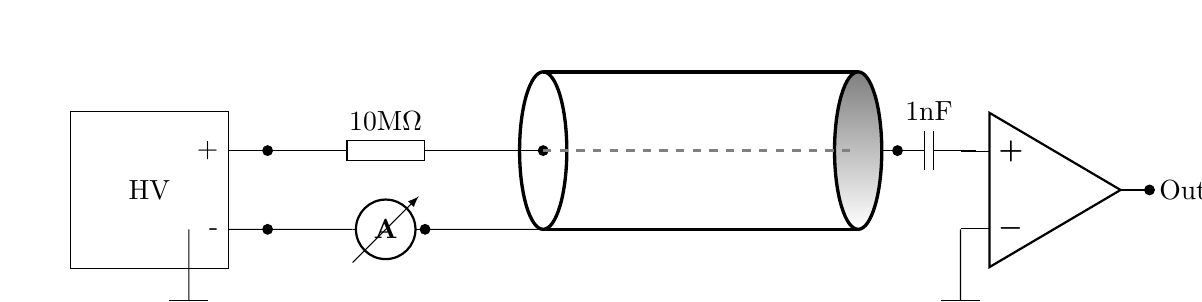
\begin{tikzpicture}[circuit ee IEC]
		\draw (0,0) rectangle (2,2);
		\node[left] at (2,0.5) {-};
		\node[left] at (2,1.5) {+};
		\node[] at (1,1) {HV};
		\draw (1.5,.5) to [ground={pos=1}] (1.5,-0.5);		
		
		\draw (2,1.5) to [resistor={ohm sloped=10M}] (6,1.5);
		\node [contact] at (2.5,1.5) {};
		\node [contact] at (6,1.5) {};
		
		\draw (2,0.5) to[ammeter] (6,.5);
		\node [contact] at (2.5,.5) {};
		\node [contact] at (4.5,.5) {};
		
%		\draw (5,.5) to [ground={pos=1}] (5,-0.5);
		
		\draw[very thick] (6,2.5) -- (10,2.5);
		\draw[very thick] (6,1.5) ellipse (0.3 and 1);
		\draw[very thick] (6,0.5) -- (10,0.5);
		\draw[very thick,shade] (10,1.5) ellipse (0.3 and 1);
		\draw[very thick, dashed, gray] (6,1.5) -- (10,1.5);
		
		\node [contact] at (10.5,1.5) {};
		\draw (10.3,1.5) to [capacitor={farad sloped=1n}] (11.5,1.5);
		
		\draw (12.5,1) node[op amp,yscale=-1] (opamp2) {};
		\draw (11.3,.5) to [ground={pos=1}] (11.3,-0.5);
		
%	amplifier with describing
%		\draw (3,0) node[op amp,yscale=-1] (opamp2) {}
%			(opamp2.+) node[left ] {$v_+$}
%  			(opamp2.-) node[left ] {$v_-$};
		
		\node [contact] at (13.7,1) {};
		\node[right] at (13.7,1) {Out};
	\end{tikzpicture}
	\caption{The electric scheme of the drift tube connection }
	%\caption{Електронна схема підключення тестового зразка дрейфової трубки}
	\label{fig:electricCircuit}	
	\end{figure}
	
	As it is seen above, the scheme is very simple.
	
	For our research we used a source $Fe^{55}$ which is suitable for a drift tube calibration. In our case $Fe^{55}$ serves as a photon source with almost monochromatic spectra with energy 5.9 keV.
	
	The most important parameter which we have to measure is Gain $G$ (\ref{eq:gain}).
	
	The idea is to measure a charge that goes through the tube electric circuit per unit of time and then find Gain.  We assume that a current $I_0$ through the ampere meter(see fig.~\ref{fig:electricCircuit}) is constant when the radioactive source is absent. The current  is non-zero when the tube detects background particles(for example atmospheric muon flux) or when  a leakage current is present. Therefore, with the presence of a source $Fe^{55}$ all surplus of the current $\bigtriangleup I = I-I_0$ in the drift tube circuit occurs because of gamma ray detection.
	
	On the other hand, we can write $\bigtriangleup I$ in terms of initial amount of electrons and Gain in the following form :
	
	\begin{equation}
	\bigtriangleup I = G N_0 e,
	\label{eq:IGainN0}
	\end{equation}
	
	where $G$ -- Gain; $N_0$ - number of initial electron-ion pairs per second; e - charge of electron in C.
	
	On the other hand we can express $N_0$ as:

	\begin{equation}
	N_0 = R \cdot \mean{n} = R \cdot\sum_n n p(n) \approx R \int_0^\infty n p(n) dn;
	\end{equation}

	where  $p(n)$ is a probability that the photon with energy 5.9 keV after interaction with argon atom will create $n$ electron-ion pairs; R is a rate [Hz], as we need to find the amount of electron-ion pairs per one second.

	The calculation of the distribution 	$p(n)$  in GARFIELD is shown in Fig.\ref{fig:n_probability}. In the figure we can the two peaks: the main photopeak and the smaller escape peak. 
%	Тут $p(n)$ - імовірність того, що фотон з енергією 5.9 КеВ провзаємодівши з атомом аргону утворить $n$ електрон іонних пар, R - частоса реєстрації сигналів [Hz] так як нам потрібно знайти кількість електрон-іонних пар за час 1с.	
%	Розрахунок розподілу $p(n)$ в GARFIELD подано на рисунку \ref{fig:n_probability}. Як видно з рисунку в розподілі $p(n)$ присутньо 2 піки: основний фотопік, та менший escape peak. 
	The escape peak for argon is known to be 3.2 keV less than the primary peak. An escape peak is formed by a number of photon interactions in the gas resulting in one primary ionization electron and a re-emitted X-ray with a long mean free path.
	
	\begin{figure}[!h]
	\centering
	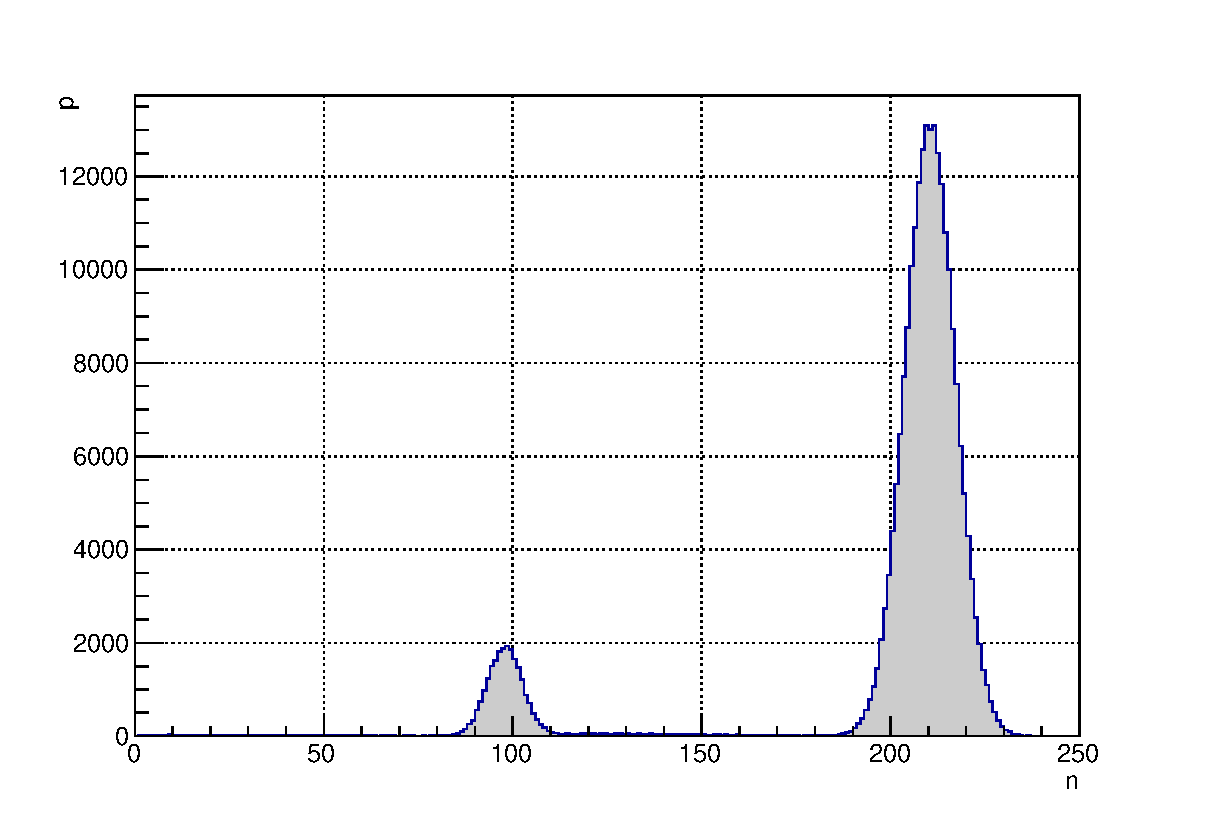
\includegraphics[width=0.7\textwidth]{fe55neGamma}
	\caption{ p(n) distribution}
%	\caption{ Розподіл актів взаємодії фотонів енергії 5.9 кеВ з газом Аргону від кількості первинних електронів, утворених в об’ємі дрейфової трубки}
	\label{fig:fe55_n_probability}
	\end{figure}
	
	The realisation of a measurement is very simple.  On the amplifier output (see Fig.\ref{fig:electricCircuit}) the signal goes to the discriminator with  trigger threshold on the level enough for a signal detection and big enough for noise neglecting. The signal from discriminator in rectangular form goes into counter. The counter is triggered for the rising edge. This scheme has a small dead time $~0.5 \mu s$, therefore for the signal frequency of $R \sim 5000 \frac{events}{second} \approx 200 \frac{\mu s}{event}$ the amount of non counted signals is negligibly small.
	
	For the first gain estimation we assume about avalanche superposition and linear amplitude dependence of final signal on the amount of initial electrons(later we will show that this is not true).
	
	From the distribution in Fig.\ref{fig:fe55_n_probability} we can find $\mean{n} = 197.87$ for average amount of primary electron because of photon (5.9keV) interaction with atoms of a gas $Ar70\%+CO_230\%$.
	
	The results of measurements are shown in the table \ref{table:GainTotal}. The Gain curves G(V) for several pressure values are shown in the Fig.\ref{fig:Gain_multy}.
		
%	Постановка експерименту виглядає досить примітивно. На виході з підсилювача (див рис.\ref{fig:electricCircuit}) сигнал подається на дискримінатор з порогом спрацьовування виставленим на рівні достатньому для реєтрації сигналів але достньо високим, щоб шум не зараховувався. Сигнал з дискримінатора у вигляді прямокутного сигналу подається на лічильних, який спрацьовує по зростаючому фронту. Така схема має малий мертвий час порядку $0.5 \mu s$, тому для частоти сигналів $R \sim 5000 \frac{events}{second} \approx 200 \frac{\mu s}{event}$ кількість незарахованих сигналів буде нищівно мала.
	
%	Для першої оцінки коефіцієнту підсилення ми припускаємо про таку собі суперпозицію лавин і лінійну маштабованість амплітуди кінцевого сигналу від кількості початкових електронів(далі ми покажемо що це не так).
	
%	З розподілу на рис.\ref{fig:fe55_n_probability} знаходимо $\mean{n} = 197.87$ для середньої кількість первинних електронів від акту взаємодії фотону енергії $5.9 keV$ з атомами газу  $Ar70\%+CO_230\%$.
	
%	Результати вимірювань представимо у вигляді таблиці \ref{table:GainTotal}. Криві коефіцієнту підсилення G(V) для ряду значень тиску зображено на рис.
	
%	Для обрахунку сигналу спершу розглянемо специфіку взамодії гамма-квантів з енергією 5.9 КеВ з Аргоном.
	
	\begin{table}[!h]
	\centering
	\begin{tabular}{|l|l|l|l|l|l|l|}
		\hline
		Gain(no cor) & P[bar] (U[V]) & HV [V] & Thr [mV]&  I [nA] & RMS [nA] & Rate [Hz]  \\
		\hline
		11138 & 1.0(0.857) & 1600 & &  1.7700 & 0.0919 & = \\
		\hline
		18196 & 1.0(0.857) & 1650 & &  2.8915 & 0.1598 & = \\
		\hline
		29255 & 1.0(0.857) & 1700 & 32 & 4.6490 & 0.2328 & 4965.9 \\
		\hline
		47012 & 1.0(0.858) & 1750 & & 7.4707 & 0.4380 & = \\
		\hline
		73159 & 1.0(0.857) & 1800 & & 11.6257 & 0.5630 & = \\
		\hline
		
		& & & & & & \\
		\hline
		
		9885 & 1.106(0.906) & 1650 & & 1.6921 & 0.1099 & = \\
		\hline
		15747 & 1.106(0.905)& 1700 & & 2.6955 & 0.13381 & = \\
		\hline
		25275 & 1.106(0.905)& 1750 & 32 & 4.3263 & 0.1975 & 5349.0 \\
		\hline
		39887 & 1.106(0.906)& 1800 & & 6.8274 & 0.2841 & = \\
		\hline
		61359 & 1.106(0.906)& 1850 & & 10.5028 & 0.4567 & = \\
		\hline
		
		& & & & & & \\
		\hline
		
		9260 & 1.205(0.951) & 1700  & & 1.6921 & 0.1053 & \\
		\hline
		14536 & 1.205(0.951) & 1750 & & 2.6562 & 0.1274 & \\
		\hline
		22991 & 1.205(0.951) & 1800 & 32 & 4.2012 & 0.1900 & 5710 \\
		\hline
		35777 & 1.205(0.951) & 1850 & & 6.5376 & 0.2880 & \\
		\hline
		54684 & 1.205(0.951) & 1900 & & 9.9924 & 0.5284 & \\
		\hline
		
		& & & & & & \\
		\hline
		
		5444 & 1.309 (0.998) & 1700 &  & $1.03 $ & $ 0.06 $ & \\
		\hline
		8351 & 1.309 (0.998) & 1750 &  & $1.58 $ & $ 0.14$ & \\
		\hline
		13267 & 1.309 (0.998) & 1800 &  & $2.51 $ & $ 0.12 $ & \\
		\hline
		20615 & 1.309 (0.998) & 1850 & 32 & $3.90 $ & $ 0.15 $ & 5987 \\
		\hline
		31716 & 1.309 (0.998) & 1900 &  & $6.00 $ & $ 0.29 $ & \\
		\hline
		48102 & 1.309 (0.998) & 1950 &  & $9.10 $ & $ 0.38 $ & \\
		\hline
		69987 & 1.309 (0.998) & 2000 &  & $13.24 $ & $ 0.50 $ & \\
		\hline
		100751 & 1.309 (0.998) & 2050 &  & $19.06 $ & $ 0.78 $ & \\
		\hline
		
	\end{tabular}
	\caption{Gain measurements}
%	\caption{Виміри коефіцієнту підсилення трубки}
	\label{table:GainTotal}
	\end{table}
	
	\begin{figure}[!h]
	\centering
	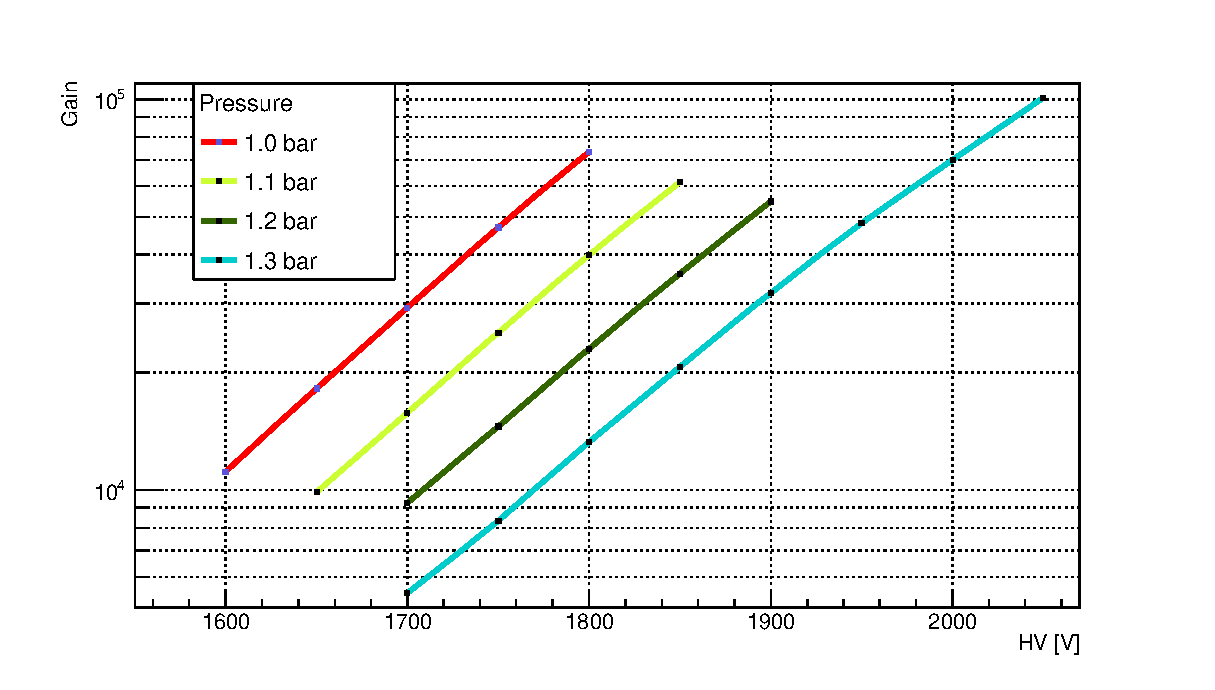
\includegraphics[width=1.0\textwidth]{gain_multyGraph}
	\caption{Gain experimental curves for several values of gas pressure in the drift tube.}
%	\caption{ Експериментальні криві коефіцієнту підсилення для набору значень тиску в дрейфовій трубці}
	\label{fig:Gain_multy}
	\end{figure}
		
	
	\subsection{Experimental spectra from the source Fe55}
		
	$^{55}Fe$  is a source of gamma-rays with energy of 5.9 keV. Each signal at the output of amplifier differs by amplitude in dependence of initial electron number. Therefore, according to the calculated in GARFIELD spectra $p(n)$ (see Fig.\ref{fig:fe55_n_probability}), it is expected to see two peaks in experimental spectra.
	
	For spectra measurements we first have to get a match between a certain signal and the amplitude on the output of the drift tube. In our case such a quantity is an integral from a signal on during the time of a signal.
	
	The amplified signal from the output of the amplifier is sent in parallel through the linear splitter to the discriminator and delay system. With the signal from discriminator the sampling signal and busy signal is formed. During the busy signal the analysing system does not accept the signal from the drift tube (this is a dead time for this detector system). The delayed signal from the amplifier integrates during the sampling signal and then digitalizes with 10-bit ADC. After digitalizing the signal is sent through the optical channel to PC, where the data is recorded into separate ROOT-file.
	
	The stages {\it sampling + storing} are time-consuming and a dead time in this case is bigger than an average time interval between events in the tube(with current detector system) therefore is a big probability to miss detecting an event.
	
	The sampling stage is built in such a way to calibrate for pedestal shelf voltage from the integrator. On the final histogram it will look as a small peak. We will calibrate exactly with regard to it. The second control point is a gamma-ray 5.9 keV photo peak from the source $^{55}Fe$.
	
	\begin{figure}
	\centering
	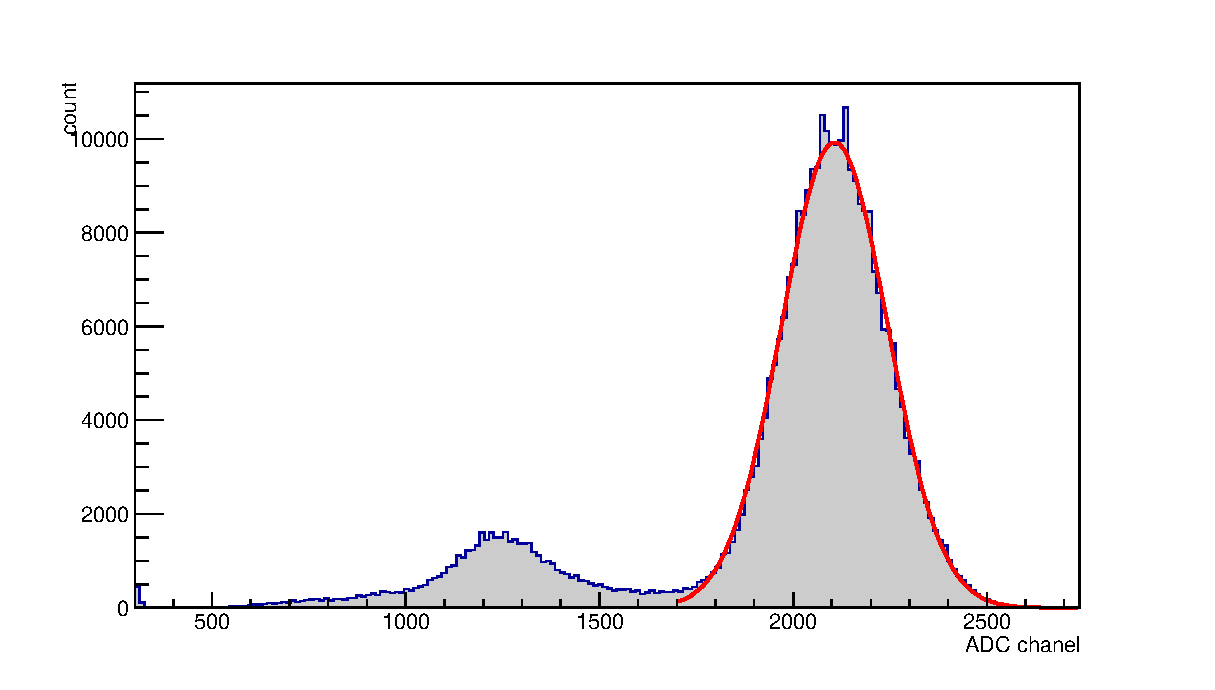
\includegraphics[width=0.7\textwidth]{expFitted1750}
	
	\caption{Experimental spectra from $^{55}Fe$.}
	\label{fig:expFitted1750}
	\end{figure}
	
%	$Fe^{55}$ - по суті є джерелом гама-квантів з енергією 5.9 КеВ. На практиці  очікуємо побачити 2 піки відповідно до симуляції(дивись рис. \ref{fig:fe55_n_probability}).
	
%	Для того, щоб вести мову про спектр спершу необхідно кожному сигналу привести у відповідність число яке лінійно залежало би від амплітуди сигналу на виході з трубки. В нашому випадку такою величиною є інтеграл від сигналу вздовж часу порядку протяжності сигналу.
	
%	Підсилений сигнал на виході з підсилювача через через лінійний розгалуджувач  паралельно пускається на дискримінатор та систему затримки. З сигналу від дискримінатора формує сигнал для вибірки сигналу, а також сигнал busy, впродовж якого аналізуча система не приймає сигнал(по суті це є мертвим часом даної детекторної установки). Затриманий сигнал від підсилювача інтегрується протягомі sampling signal і оцифровуєтсья 10 бітним АЦП. Оцифрований сигнал через оптичний канал посилається на ПК де дані гістограмуються в окремий root-файл.
	
%	Процес sampling + storing досить часо затратний, і мертвий час в даному випадку є більший за середню відстань між подіями в трубці, тому є велика імовірність пропустити події.
	
%	Етап самплінгу побудований таким чином, що дозволяє відкалібрувати сигнал для випадку відсутності сигналу в трубці. На кінцевій гістограмі це виливаєтсья в маленький пік. Відносно нього ми і будемо калібруватися. Другою реперною точкою в нас буде фотопік від gamma квантів 5.9 КеВ джерела $Fe^{55}$.
	
	\begin{table}[!h]
	\centering
	\begin{tabular}{|l|r|l|}
		\hline
		point of reference & channel & electrons per cluster(simulations)\\
		\hline
		zero pedestal ($gauss~\mu \pm \bigtriangleup \mu)$ & $301.1 \pm 0.3 $ & 0\\
		\hline
		$5.9~keV$ & $2107.4 \pm 0.3$ & $210.42 \pm 0.01$ \\ 
		\hline
		escape peak & $1253.3 \pm 0.9 $ & $97.99 \pm 0.03$ \\
		\hline
	\end{tabular}
	\caption{ Coordinates of peaks from Fig.\ref{fig:expFitted1750} and Fig.\ref{fig:fe55_n_probability}}
%	\caption{ Координати центрів піків на симуляціях(в одиницях кількості електронів на подію) та спектр зі спектрометра (вихід 12 бітного АЦП)}
	\label{table:peakPos}
	\end{table}
	
	\subsection{ Space charge effect}
	
	Photons from $^{55}Fe$ of energy 5.9 keV create $\sim 200$ electron-ion pairs as a result of photoeffect with $Ar70\%+CO_230\%$ gas mixture. As we have a strong electric field between anode and cathode such electron cloud starts to drift toward a wire. The external field distorts as any space charge creates its own e/m field. As a result, partial avalanches per initial electron of a cloud creates an avalanche of size smaller than from a single-electron cloud(as in case muon ionisation).
	
	Such an effect indeed was observed. If we suppose a linear dependence of output signal amplitude from number of initial electrons a relative position for experimental peak should be located at(calibration relatively to the photopeak):
	
	\begin{equation}
			channel_{escapePeak} = \frac{2107.4 - 301.1}{210.42} 98 + 301.1 = 1142.3 \ne 1253.3,
	\end{equation}

	
\newpage
\section{Appendix}

\subsection{pressure meter}

	For the pressure measurement inside of drift tube we used pressure transmitters from SensorTechnics$^{\textregistered}$. The devise is marked by ID:CTE9005AQ4, so we used appropriate datasheet  from the manufacturer \cite{presTransmitDatasheet}.
	
	According to datasheet and marking, this pressure transmitter is designed for pressure measurements in the interval $0 \dots 5~bar$. But on the transmitter is marked an interval $0\dots 3,5~bar$. So to be able to use this device, we additionally calibrated it.
	
	For this purpose we used two control points: the output current value for atmospheric pressure at that point (727 mmHg) and a current for a vacuum. To get a vacuum we used a pump which decreases a pressure to the value  $<0.001~bar$ which we consider as a vacuum.
	
%	Для вимірювання тиску в дрейфовій трубці використовувався датчик тиску(pressure transmitters) від компанії SensorTechnics$^{\textregistered}$. На приладі зазначено ідентифікаційний код ID:CTE9005AQ4, по якому було знайдено відповідну документацію від виробника \cite{presTransmitDatasheet}.

%	Згідно до документації та маркування, даний прилад розрахований на вимірювання тиску в діапазоні від $0 \dots 5~bar$. Проте безпосередньо на самому манометрі вказаний діапазон $0\dots 3,5~bar$. Тож для використання даного приладу ми вдалися до додаткової калібровки.
	
%	Для досягнення даної цілі було використано 2 контрольні точки: показник струму для атмосферного тиску в даний момент, і струм для вакууму. Для досягнення вакууму була використана помпа що понижувала тиск до значення $<0.001~bar$ що можна вважати за вакуум.
	
	\begin{table}[!h]
	\centering
	\caption{ Control points for calibration of pressure transmitter.}
	\begin{tabular}{|l|l|}
		\hline
		pressure [bar] & voltage[V] \\
		\hline
		$<0.001$ & 0.405\\
		\hline
		1 & 0.858\\
		\hline
	\end{tabular}
	\end{table}
	
	Therefore the voltage dependence taken on a resistor 	$100\Omega$ depends on a pressure as:
%	Таким чином залежність напруги що знімається на резистрорі $100\Omega$ залежить від тиску по закону:
	\begin{equation}
	V = 4.05 + 0.453 \cdot P[bar]
	\end{equation}

	\begin{equation}	
	P[bar] = -0.894 + 2.2075 \cdot V
	\end{equation}

\newpage
\begin{thebibliography}{00}	
		
	\bibitem{NA62_TDR} F. Hahn, F. Ambrosino, A. Ceccucci, H. Danielsson, N. Doble, F. Fantechi, A. Kluge, C. Lazzeroni, M. Lenti, G. Ruggiero, M. Sozzi, P. Valente, and R. Wanke. NA62: Technical Design Document. Technical Report NA62-10-07, CERN, Geneva
	
	\bibitem{ship_TP} SHiP Technical Proposal from 8 april 2015: arXiv:1504.04956v1
	
	\bibitem{garfield} GARFIELD tutorial \url{http://garfield.web.cern.ch/garfield}
	
	\bibitem{kozlinskiy} Outer Tracker calibration and open charm production cross section measurement at LHCb, 2013 A.V.Kozlinskiy. \\  \url{http://dspace.ubvu.vu.nl/bitstream/handle/1871/40430/dissertation.pdf}
	
	\bibitem{presTransmitDatasheet} DataSheet for Pressure transmitters for corrosive liquids and gases CTE/CTU9000 series. \url{http://www.first-sensor.com/cms/upload/datasheets/DS_Standard-CTE-CTU9000_E_11509.pdf}
	
	\bibitem{EoI} W. Bonivento, A. Boyarsky, H. Dijkstra, U. Egede, M. Ferro-Luzzi, B. Goddard, A. Golutvin, D. Gorbunov, R. Jacobsson, J. Panman, M. Patel, O. Ruchayskiy, T. Ruf, N. Serra, M. Shaposhnikov, and D. Treille. Proposal to Search for Heavy Neutral Leptons at the SPS. Technical Report CERN-SPSC-2013-024. SPSC-EOI-010, CERN, Geneva (Oct, 2013).
	
\end{thebibliography}
	
\end{document}
